\documentclass[11pt,oneside]{article}	%use"amsart"insteadof"article"forAMSLaTeXformat
\usepackage{geometry}		%Seegeometry.pdftolearnthelayoutoptions.Therearelots.
\geometry{letterpaper}		%...ora4paperora5paperor...
%\geometry{landscape}		%Activateforforrotatedpagegeometry
%\usepackage[parfill]{parskip}		%Activatetobeginparagraphswithanemptylineratherthananindent
\usepackage{graphicx}				%Usepdf,png,jpg,orepswithpdflatex;useepsinDVImode
								%TeXwillautomaticallyconverteps-->pdfinpdflatex		
\usepackage{amssymb}
\usepackage[colorlinks]{hyperref}

%----macros begin---------------------------------------------------------------
\usepackage{color}
\usepackage{amsthm}
\usepackage{amsmath}

\def\conv{\mbox{\textrm{conv}\,}}
\def\aff{\mbox{\textrm{aff}\,}}
\def\E{\mathbb{E}}
\def\R{\mathbb{R}}
\def\Z{\mathbb{Z}}
\def\tex{\TeX}
\def\latex{\LaTeX}
\def\v#1{{\bf #1}}
\def\p#1{{\bf #1}}
\def\T#1{{\bf #1}}

\def\vet#1{{\left(\begin{array}{cccccccccccccccccccc}#1\end{array}\right)}}
\def\mat#1{{\left(\begin{array}{cccccccccccccccccccc}#1\end{array}\right)}}

\def\lin{\mbox{\rm lin}\,}
\def\aff{\mbox{\rm aff}\,}
\def\pos{\mbox{\rm pos}\,}
\def\cone{\mbox{\rm cone}\,}
\def\conv{\mbox{\rm conv}\,}
\newcommand{\homog}[0]{\mbox{\rm homog}\,}
\newcommand{\relint}[0]{\mbox{\rm relint}\,}

%----macros end-----------------------------------------------------------------

\title{Hypercuboidal grids and topological products in LARCC
\footnote{This document is part of the \emph{Linear Algebraic Representation with CoChains} (LARCC) framework~\cite{cclar-proj:2013:00}. \today}
}
\author{LARCC team}
%\date{}							%Activatetodisplayagivendateornodate

\begin{document}
\maketitle
\nonstopmode

\begin{abstract}
Here we develop an efficient implementation of multidimensional grid generation of cuboidal and simplicial cell complexes, and a fast implementation of the more general Cartesian product of cellular complexes. Both kind of operators, depending on the dimension of their input, may generate either full-dimensional (i.e.~solid) output complexes or cellular complexes of dimension $d$ embedded in Euclidean space of dimension $n$, with $d\leq n$. 
\end{abstract}

\tableofcontents
\newpage

\section{Introduction}

This report aims to discuss the design and the implementation of the \texttt{largrid} module of the LAR-CC library, including also the Cartesian product of general cellular complexes. 
In particular, we show that both $n$-dimensional grids of (hyper)-cuboidal cells and their  $d$-dimensional skeletons ($0\leq d\leq n$), embedded in $\E^n$, may be properly and efficiently generated by assembling the cells produced by a number $n$ of either $0$- or $1$-dimensional cell complexes, that in such lowest dimensions coincide with simplicial complexes. 

In Section~\ref{sec:0-1-complexes} we give the simple implementation of generation of lower-dimensional (say, either 0- or 1-dimensional) regular cellular complexes with integer coordinates.
In Section~\ref{sec:cuboids} a functional decomposition of the generation of either full-dimensional cuboidal complexes in $\E^n$ and of their $d$-skeletons ($0\leq d\leq n$) is given, showing in particular that every skeleton can be efficiently generated as a partition in cell subsets produced by the Cartesian product of a proper disposition of 0-1 complexes, according to the binary representation of a subset of the integer interval $[0,2^n]$.
In Section~\ref{sec:product} we provide a very simple and general implementation of the topological product of \emph{two} cellular complexes of any topology. When applied to embedded linear cellular complexes (i.e.~when the coordinates of 0-cells of arguments are fixed and given) the algorithm produces a Cartesian product of its two arguments.
In Section~\ref{sec:largrid} the exporting of the module to different languages is provided.
The Section~\ref{sec:tests} contains the unit tests associated to the various algorithms, that are exported by the used literate environment in the proper test subdirectory---depending on the implementation language.
In Section~\ref{sec:indices} the indexing structure of the macro sources and variables is exposed by the sake of the reader. 
The Appendix~\ref{sec:utilities} contains some programming utilities possibly needed by the developers.

\section{0D- and 1D-complexes}
\label{sec:0-1-complexes}

We are going to use 0- and 1-dimensional cell complexes as the basic material for several operations, including generation of simplicial and cellular grids and topological and Cartesian product of cell complexes. 


\subsection{Generation of cells}

\paragraph{Uniform 0D complex}
The \texttt{grid0} second-order function generates a 0-dimensional uniform complex embedding $n+1$ equally-spaced (at unit intervals) 0-cells within the 1D interval. It returns the cells of this 0-complex.

%-------------------------------------------------------------------------------
@d Generation of uniform 0D cellular complex 
@{def grid0(n):
    cells = AA(LIST)(range(n+1))
    return cells
@}
%-------------------------------------------------------------------------------

\paragraph{Uniform 1D complex}
A similar \texttt{grid1} function returns a uniform 1D cellular complex with $n$ 1D \texttt{cells}.

%-------------------------------------------------------------------------------
@d Generation of uniform 1D cellular complex 
@{def grid1(n):
    ints = range(n+1)
    cells = TRANS([ints[:-1],ints[1:]])
    return cells
@}
%-------------------------------------------------------------------------------

\paragraph{Uniform 0D or 1D complex}
A \texttt{larGrid} function is finally given to generate the LAR representation of the cells of either a 0- or a 1-dimensional complex, depending on the value of the \texttt{d} parameter, to take values in the set $\{0,1\}$, and providing the \emph{order} of the output complex.
%-------------------------------------------------------------------------------
@d Generation of cellular complex of 0/1 dimension $d$
@{def larGrid(n):
    def larGrid1(d):
        if d==0: return grid0(n)
        elif d==1: return grid1(n)
    return larGrid1
@}
%-------------------------------------------------------------------------------


\subsection{Generation of embedding vertices}

\paragraph{Generation of grid vertices}
The second-order \texttt{larSplit} function is used to subdivide the real interval $[0,dom]$ into $n$ equal parts. It returns the list of $n+1$ \texttt{vertices} 1D of this decomposition, each represented as a singleton list. 

%-------------------------------------------------------------------------------
@d Generation of vertices of decompositions of 1D intervals 
@{def larSplit(dom):
    def larSplit1(n):
        # assert n > 0 and isinstance(n,int)
        item = float(dom)/n
        ints = range(n+1)
        items = [item]*(n+1)
        vertices = [[int*item] for (int,item) in zip(ints,items)]
        return vertices
    return larSplit1
@}
%-------------------------------------------------------------------------------


\section{Cuboidal grids}
\label{sec:cuboids}

More interesting is the generation of \emph{hyper-cubical grids} of intrinsic dimension $d$ embedded in $n$-dimensional space, via the Cartesian product of $d$ 1-complexes and $(n-d)$ 0-complexes. When $d=n$ the resulting grid is said \emph{solid}; when $d=0$ the output grid is 0-dimensional, and corresponds to a grid-arrangement of a discrete set of points in $\E^n$.


\subsection{Full-dimensional grids}

\subsubsection{Vertex generation}

First the grid vertices are produced by the \texttt{larVertProd} function, via Cartesian product of vertices of the $n$ 1-dimensional arguments (vertex lists in \texttt{vertLists}), orderly corresponding to $x_0$, $x_1$, ..., $x_{n-1}$ in the output points $(x_0, x_1,\ldots,x_{n-1})$.
%-------------------------------------------------------------------------------
@d Generation of grid vertices 
@{def larVertProd(vertLists):
    return AA(CAT)(CART(vertLists))
@}
%-------------------------------------------------------------------------------


\subsubsection{Mapping of indices to storage}

\paragraph{Multi-index to address transformation}
The second-order utility \texttt{index2addr} function transforms a \texttt{shape} list for a multidimensional array into a function that, when applied to a multindex array, i.e.~to a list of integers within the \texttt{shape}'s bounds, returns the integer address of the array component within the linear storage of the multidimensional array.

The transformation formula for a $d$-dimensional array with \texttt{shape} $(n_0,n_1,...,n_{d-1})$ is a linear combination of the 0-based\footnote{0-based array, like in C, java and python, as opposed to 1-based, like in fortran or matlab.} multi-index $(i_0,i_1,...,i_{d-1})$ with \texttt{weights} equal to $(w_0,w_1,...,w_{d-2},1)$:
\[
addr = i_0\times w_0 +i_1\times w_1 +\cdots +i_{d-1}\times w_{d-1}
\]
where 
\[
w_k = n_{k+1} \times n_{k+2} \times\cdots\times  n_{d-1}, \qquad 0\leq k\leq d-2.
\]

Therefore, we get $\texttt{index2addr([4,3,6])([2,2,0])}=48= 2\times(3\times 6)+2\times(6\times 1)+0$,
where \texttt{[2,2,0]} represent the numbers of (pages, rows, columns) indexing an element in the three-dimensional array of shape \texttt{[4,3,6]}.

%-------------------------------------------------------------------------------
@d Transformation from multindex to address in a linear array storage
@{def index2addr (shape):
    n = len(shape)
    shape = shape[1:]+[1]
    weights = [PROD(shape[k:]) for k in range(n)]
    def index2addr0 (multindex):
        return INNERPROD([multindex, weights])
    return index2addr0
@}
%-------------------------------------------------------------------------------

\paragraph{\texttt{index2addr} examples}
In the following example, \texttt{[3,6]} is the \texttt{shape} of a two-dimen\-sion\-al array with 3 rows and 6 columns, stored in row-major order (i.e.~by rows). The expression \texttt{index2addr([3,6])([2,0])} returns $12=2\times(6\times 1)+0$, since the array element characterised by the multi-index value \texttt{[2,0]} is addressed at position 12 (starting from 0) in the linear storage of the array. Analogously, the function \texttt{index2addr([3,6])}, when applied to all the index values addressing the array of shape \texttt{[3,6]}, produces the integers between 0 and $17 = 3\times 6 -1$. In the last example, the function \texttt{index2addr([4,3,6])} is applied to all the 0-based triples indexing a three-dimensional array of the given shape. Of course, the mapping works correctly even when the array shape is one-dimensional, as shown by the last example below.

%-------------------------------------------------------------------------------
@d Test example 
@{>>> index2addr([3,6])([2,0])
12
>>> [index2addr([3,6])(index) for index in CART([ range(3), range(6) ])]
[0, 1, 2, 3, 4, 5, 6, 7, 8, 9, 10, 11, 12, 13, 14, 15, 16, 17]
>>> convert = index2addr([4,3,6])
<function index2address0>
>>> [convert(index) for index in CART( AA(range)([4,3,6]) )]
[0, 1, 2, 3, 4, 5, 6, 7, 8, 9, 10, 11, 12, 13, 14, 15, 16, 17, 18, 19, 20, 
21, 22, 23, 24, 25, 26, 27, 28, 29, 30, 31, 32, 33, 34, 35, 36, 37, 38, 39, 
40, 41, 42, 43, 44, 45, 46, 47, 48, 49, 50, 51, 52, 53, 54, 55, 56, 57, 58, 
59, 60, 61, 62, 63, 64, 65, 66, 67, 68, 69, 70, 71]
>>> index2addr([4])([2])
2
@}
%-------------------------------------------------------------------------------

\subsubsection{Multidimensional cell generation}

In this section we discuss the implementation of the generation of cells as lists of indices to grid vertices. First, we study the case that the output complex is generated by the Cartesian product of \emph{any} number of either 0- or 1-dimensional cell complexes. Then, we discuss an efficient extraction of $d$-dimensional skeleton of a (solid) $n$-dimensional grid, for $0\leq d\leq n$.


\paragraph{Example}
In order to better understand the generation of cuboidal grids from products of 0- or 1-dimensional complexes, below we show a simple example of 2D grids embedded in $\E^3$.
In particular, \texttt{v1 = [[0.],[1.],[2.],[3.]]} and \texttt{v0 = [[0.],[1.],[2.]]} are two arrays of 1D vertices, \texttt{c1 = [[0,1],[1,2],[2,3]]} and \texttt{c0 = [[0],[1],[2]]} are the LAR representation of a 1-complex and a 0-complex, respectively. The solid 2-complex named \texttt{grid2D} given below is shown in Figure~\ref{fig:firstgrid23D}a.
\begin{align*}\scriptsize
&\texttt{grid2D = larVertProd([v1,v1]),larCellProd([c1,c1])}\\
&\texttt{VIEW(EXPLODE(1.2,1.2,1.2)(MKPOLS(grid2D)))}
\end{align*}

\begin{figure}[htbp] %  figure placement: here, top, bottom, or page
   \centering
   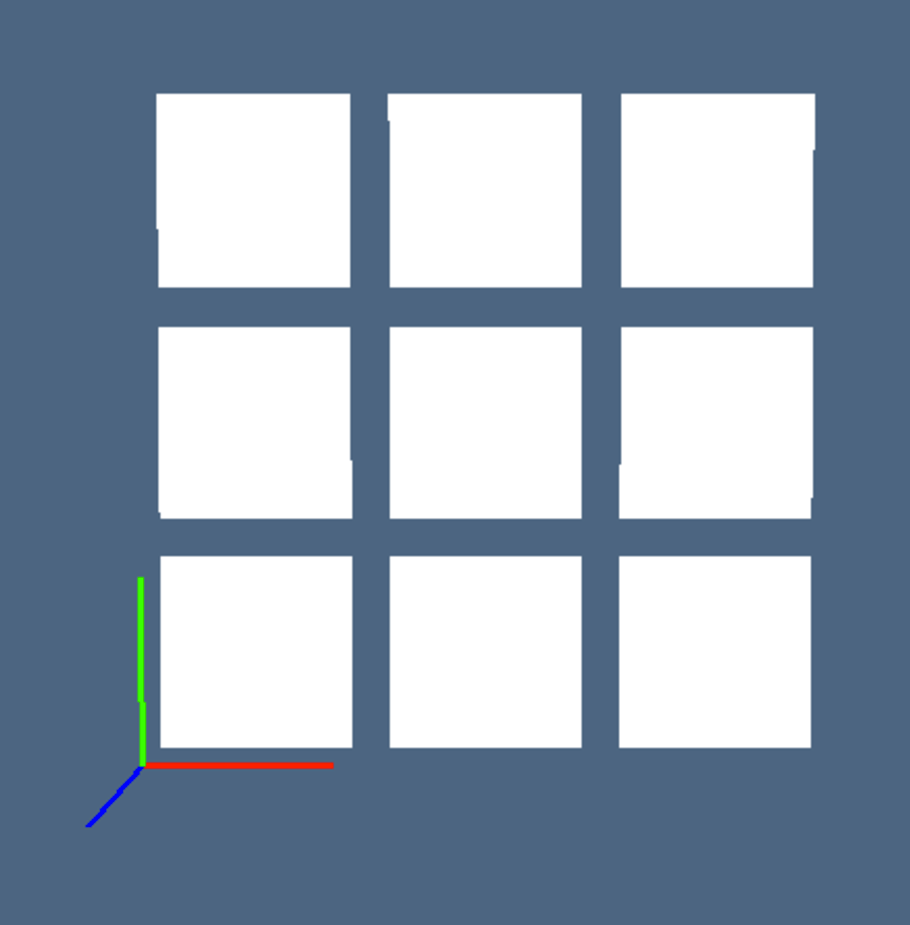
\includegraphics[width=0.458\linewidth]{images/grid2D} 
   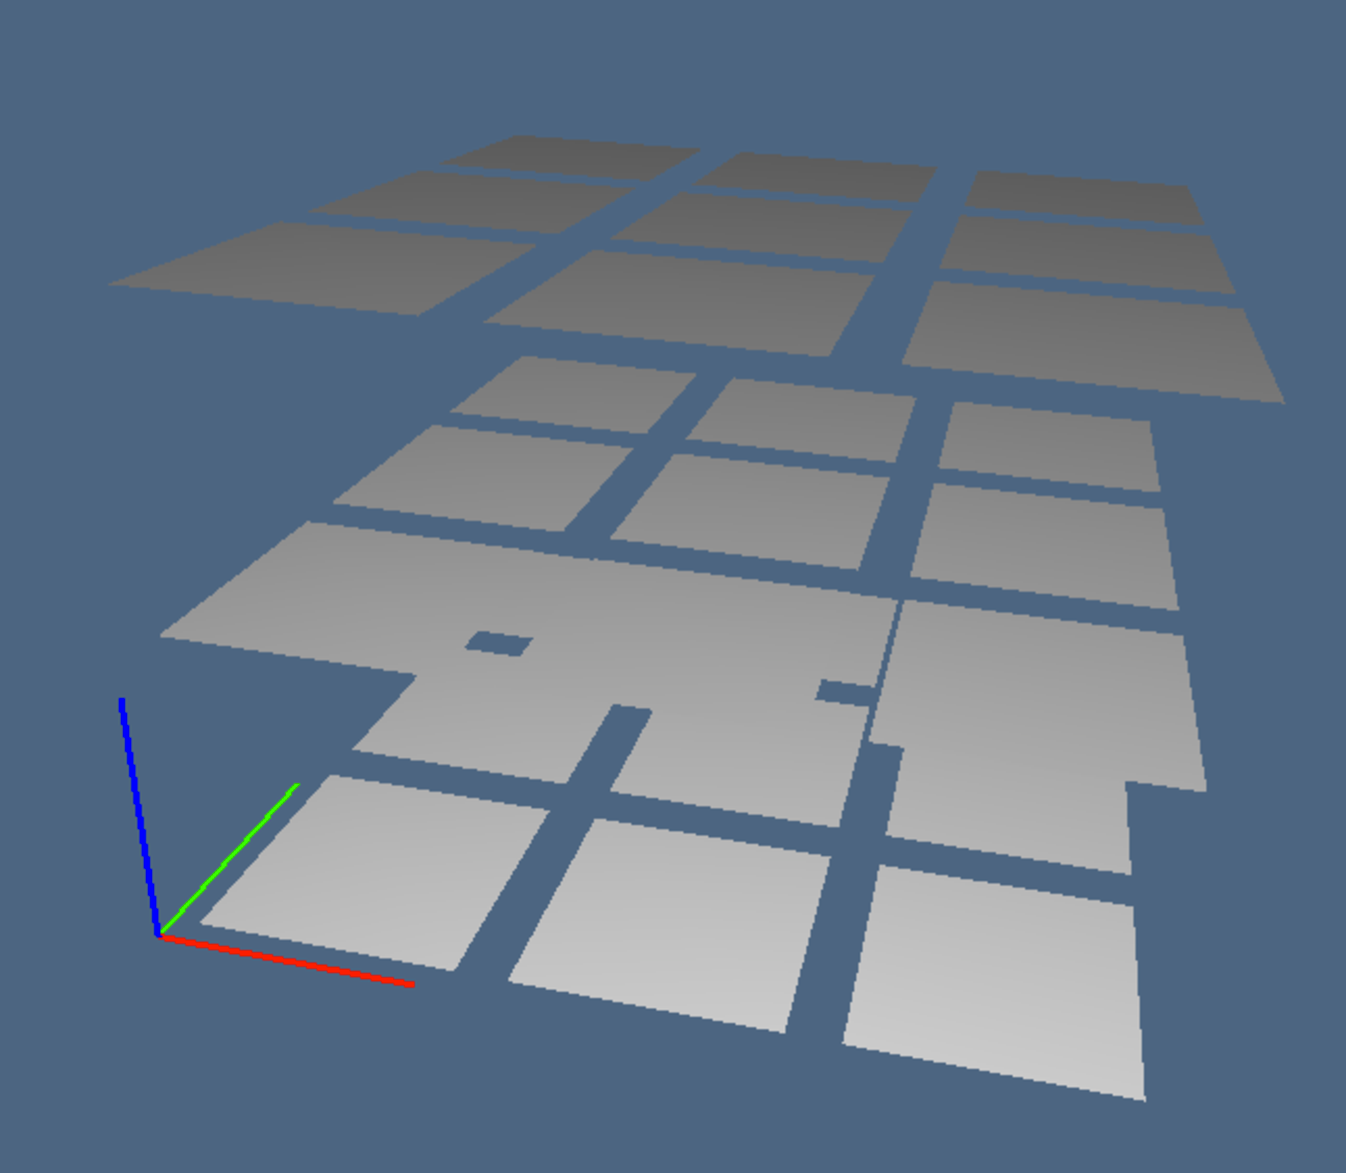
\includegraphics[width=0.532\linewidth]{images/grid3D} 
   \caption{Exploded views of models \texttt{grid2D} and \texttt{grid3D}.}
   \label{fig:firstgrid23D}
\end{figure}

Notice that \texttt{grid2D}, generated by product of two 1-complexes, is \emph{solid} in $\E^2$, whereas \texttt{grid3D} shown in Figure~\ref{fig:firstgrid23D}b, generated by product of two 1-complexes and one 0-complex, is two-dimensional and embedded in $\E^3$.

%-------------------------------------------------------------------------------
@D Example of cuboidal grid of dimensions $(2,3)$ 
@{v1, c1 = [[0.],[1.],[2.],[3.]],[[0,1],[1,2],[2,3]]
v0, c0 = [[0.],[1.],[2.]], [[0],[1],[2]]
vertGrid = larVertProd([v1, v1, v0])
cellGrid = larCellProd([c1, c1, c0])
grid3D = vertGrid,cellGrid
VIEW(EXPLODE(1.2,1.2,1.2)(MKPOLS(grid3D)))
@}
%-------------------------------------------------------------------------------

\paragraph{Cartesian product of 0/1-complexes}
Here, the input is given by the array \texttt{cellLists} of lists of cells of the argument complexes. Hence, the \texttt{shapes} variable contains the (list of) numbers $m_0, m_1, ...$ of cells in each argument complex, and the \texttt{indices} variable (generated by Cartesian product) collects the whole set $M_0 \times M_1 \times \cdots$ of 0-based multi-indices corresponding to the cells of the output complex, with $M_k = \{0,1,...,m_{k}-1\}$.

The \texttt{jointCells} variable is used to contain the list of outputs of Cartesian products of \texttt{cells} corresponding to every \texttt{index} in \texttt{indices}.

%-------------------------------------------------------------------------------
@D Generation of grid cells 
@{def larCellProd(cellLists):
    shapes = [len(item) for item in cellLists]
    indices = CART([range(shape) for shape in shapes])
    jointCells = [CART([cells[k] for k,cells in zip(index,cellLists)])
                  for index in indices]
    convert = index2addr([ shape+1 if (len(cellLists[k][0]) > 1) else shape
                             for k,shape in enumerate(shapes) ])
    return [AA(convert)(cell) for cell in jointCells]
@}
%-------------------------------------------------------------------------------

With reference to the evaluation of the expression \texttt{larCellProd([c1,c1])}, where \texttt{c1} is the LAR representation of a 1-complex with 3 cells, defined by 4 vertices (0-cells), we have the  trace given below.
Of course, the function invocation returns the list of cells of the topological product of the input complexes, each one expressed as a list of vertices of the Cartesian product of the corresponding component vertices. The partially evaluated function \texttt{index2addr0}, stored in the \texttt{convert} variable, is used to execute the mapping, for each output \texttt{cell} in \texttt{jointCells}, from vertex multi-indices to their linear storage address. The mindful reader should notice that the number of generated cells is always equal to the product of terms in \texttt{shape}, in turn equal to the number of elements in \texttt{indices} and in \texttt{jointCells}. In this case we have $|\texttt{larCellProd([c1,c1])}| = 3\times 3=9$.

%-------------------------------------------------------------------------------
@D Tracing the evaluation of expression ``\texttt{larCellProd([c1,c1])}''
@{c1 = [[0,1], [1,2], [2,3]]
cellLists = [[[0,1], [1,2], [2,3]], [[0,1], [1,2], [2,3]]]
shapes = [3,3]
indices = [[0,0], [0,1], [0,2], [1,0], [1,1], [1,2], [2,0], [2,1], [2,2]]
jointCells = [
 [[0,0], [0,1], [1,0], [1,1]],
 [[0,1], [0,2], [1,1], [1,2]],
 [[0,2], [0,3], [1,2], [1,3]],
 [[1,0], [1,1], [2,0], [2,1]],
 [[1,1], [1,2], [2,1], [2,2]],
 [[1,2], [1,3], [2,2], [2,3]],
 [[2,0], [2,1], [3,0], [3,1]],
 [[2,1], [2,2], [3,1], [3,2]],
 [[2,2], [2,3], [3,2], [3,3]]]
convert = <function index2address0>
return [
 [0,1,4,5],
 [1,2,5,6],
 [2,3,6,7],
 [4,5,8,9],
 [5,6,9,10],
 [6,7,10,11],
 [8,9,12,13],
 [9,10,13,14],
 [10,11,14,15]]
@}
%-------------------------------------------------------------------------------


\subsection{Lower-dimensional grid skeletons}

In order to compute the $d$-skeletons of a $n$-dimensional cuboidal ``grid'' complex, with $0\leq d\leq n$, let us start by remarking a similarity with the generation of the boolean representation of numbers between 0 and $2^n -1$, generated as a list of strings by the \texttt{binaryRange} function, given in Section~\ref{sec:binaryRange}.

The binary representations of such numbers are in fact filtered according to the number of their ones in Section~\ref{sec:filterByOrder}, and used to generate the distinct components of different order skeletons of the assembled grid complexes in Section~\ref{sec:assembly}.

\subsubsection{Generation of skeleton components}
\label{sec:binaryRange}

The \texttt{binaryRange} function, applied to an integer $n$, returns the string representation of all binary numerals between 0 and $2^n -1$. All the strings have the same length $n$. The bits in each strings will be used to select between either a 0- or a 1-dimensional complex as generator (via a Cartesian product of complexes) of a component of an embedded grid skeleton of proper intrinsic dimension.

%-------------------------------------------------------------------------------
@D Enumeration of binary ranges of given order
@{def binaryRange(n):
    return [('{0:0'+str(n)+'b}').format(k) for k in range(2**n)]
@}
%-------------------------------------------------------------------------------

\paragraph{Examples of generation of bit strings}
Below we show the outputs returned by application of the \texttt{binaryRange} function to the first 4 integers.
%-------------------------------------------------------------------------------
@D Binary range examples 
@{>>> print binaryRange(4),
['0000', '0001', '0010', '0011', '0100', '0101', '0110', '0111', 
 '1000', '1001', '1010', '1011', '1100', '1101', '1110', '1111']
>>> print binaryRange(3),
['000', '001', '010', '011', '100', '101', '110', '111']
>>> print binaryRange(2),
['00', '01', '10', '11']
>>> print binaryRange(1),
['0', '1']
@}
%-------------------------------------------------------------------------------

\subsubsection{Filtering grid skeleton components}
\label{sec:filterByOrder}

The function \texttt{filterByOrder} is used to partition the previous binary strings into $n+1$ subsets, such that the bits into each string sum to the same number, ranging from 0 to $n$ included, respectively.

%-------------------------------------------------------------------------------
@D Filtering binary ranges by order
@{def filterByOrder(n):
    terms = [AA(int)(list(term)) for term in binaryRange(n)]
    return [[term for term in terms if sum(term) == k] for k in range(n+1)]
@}
%-------------------------------------------------------------------------------

\paragraph{Examples of bit lists filtering}
Some examples of application of the \texttt{filterByOrder} function to the first few integers are shown below.
Of course, the number of elements in each class (i.e.~in each returned list) is ${n \choose d}$, and the total number of elements for each fixed $n$ is $\sum_{d=0}^n {n \choose d} = 2^n$.

%-------------------------------------------------------------------------------
@D Skeleton component examples 
@{>>> filterByOrder(4)
[[[0,0,0,0]],
 [[0,0,0,1], [0,0,1,0], [0,1,0,0], [1,0,0,0]],
 [[0,0,1,1], [0,1,0,1], [0,1,1,0], [1,0,0,1], [1,0,1,0], [1,1,0,0]],
 [[0,1,1,1], [1,0,1,1], [1,1,0,1], [1,1,1,0]],
 [[1,1,1,1]]]
>>> filterByOrder(3)
[[[0,0,0]],
 [[0,0,1], [0,1,0], [1,0,0]],
 [[0,1,1], [1,0,1], [1,1,0]],
 [[1,1,1]]]
>>> filterByOrder(2)
[[[0,0]], [[0,1], [1,0]], [[1,1]]]
>>> filterByOrder(1)
[[[0]], [[1]]]
@}
%-------------------------------------------------------------------------------


\subsubsection{Assembling grid skeleton components}
\label{sec:assembly}

We are now finally able to generate the various subsets of cells of a $d$-dimensional cuboidal grid skeleton, produced respectively by the expression \texttt{larCellProd(cellLists)} for every permutation of 0- and 1-complexes, according to the partition classes of permtation of $n$ bits previously produced. To understand why this assembling step of cells is necessary, the reader should look at Figure~\ref{fig:sleletons}, where three subsets of 2-cells of the 2-skeleton, respectively generated by the bit dispositions \texttt{[[0,1,1], [1,0,1], [1,1,0]]}, are separately displayed.
Notice also that, whereas the dimension $n$ of the embedding space is implicittly provided by the \texttt{length} of the \texttt{shape} parameter, the intrinsic dimension $d$ of the skeleton to be produced must be given explicitly.

\begin{figure}[htbp] %  figure placement: here, top, bottom, or page
   \centering
   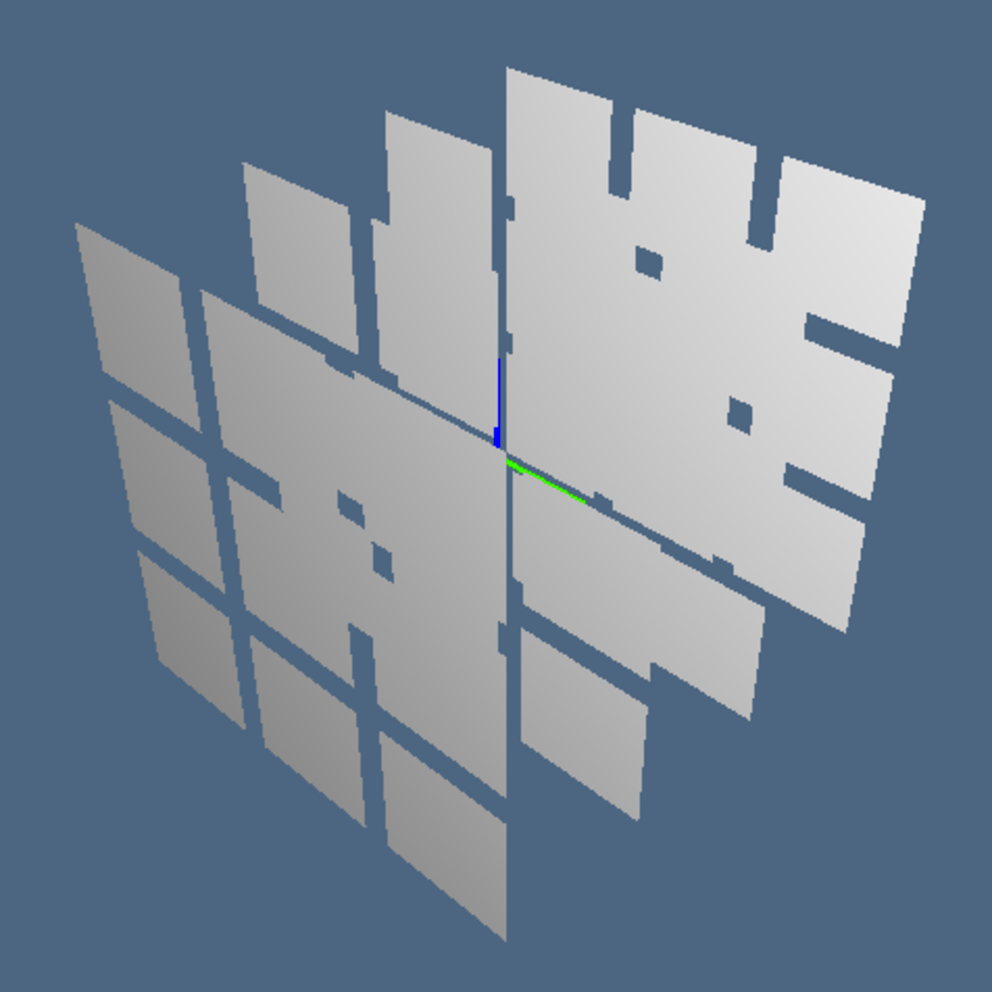
\includegraphics[height=0.245\linewidth,width=0.242\linewidth]{images/skel2a} 
   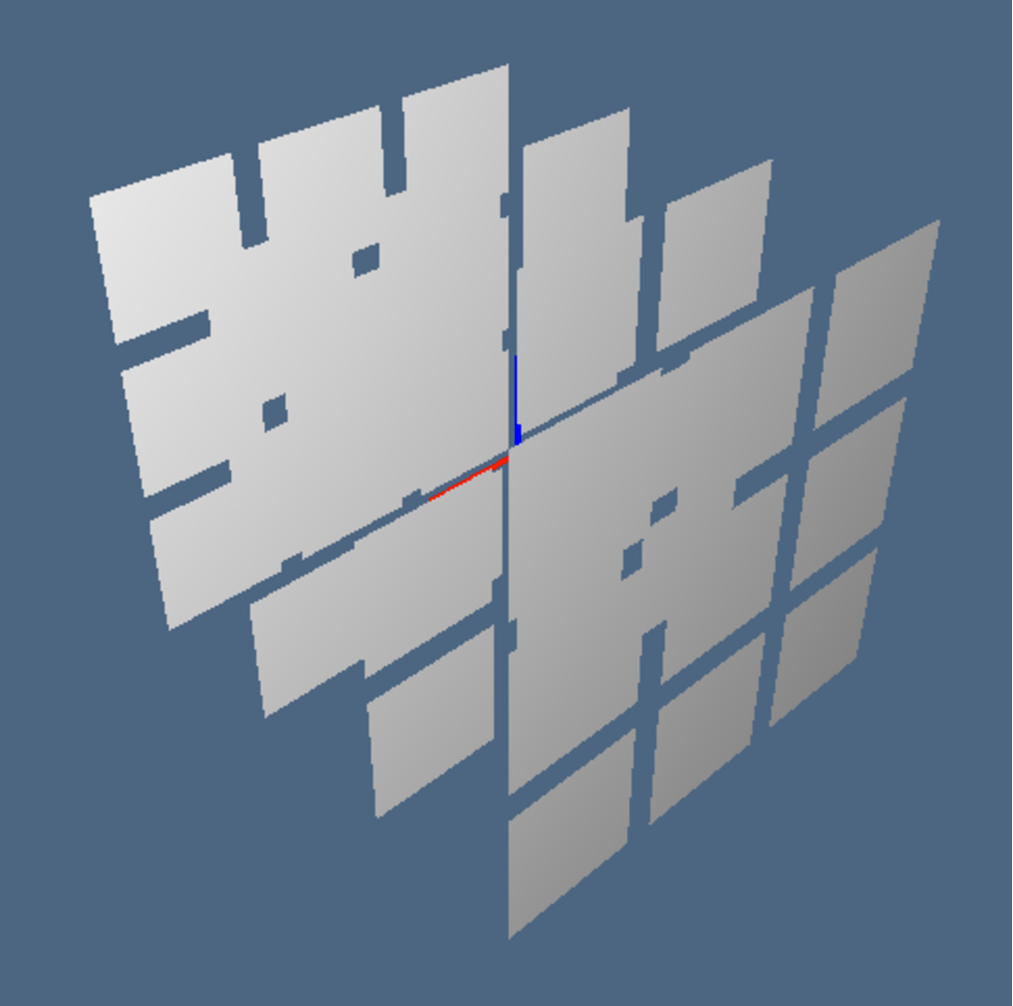
\includegraphics[height=0.245\linewidth,width=0.242\linewidth]{images/skel2b} 
   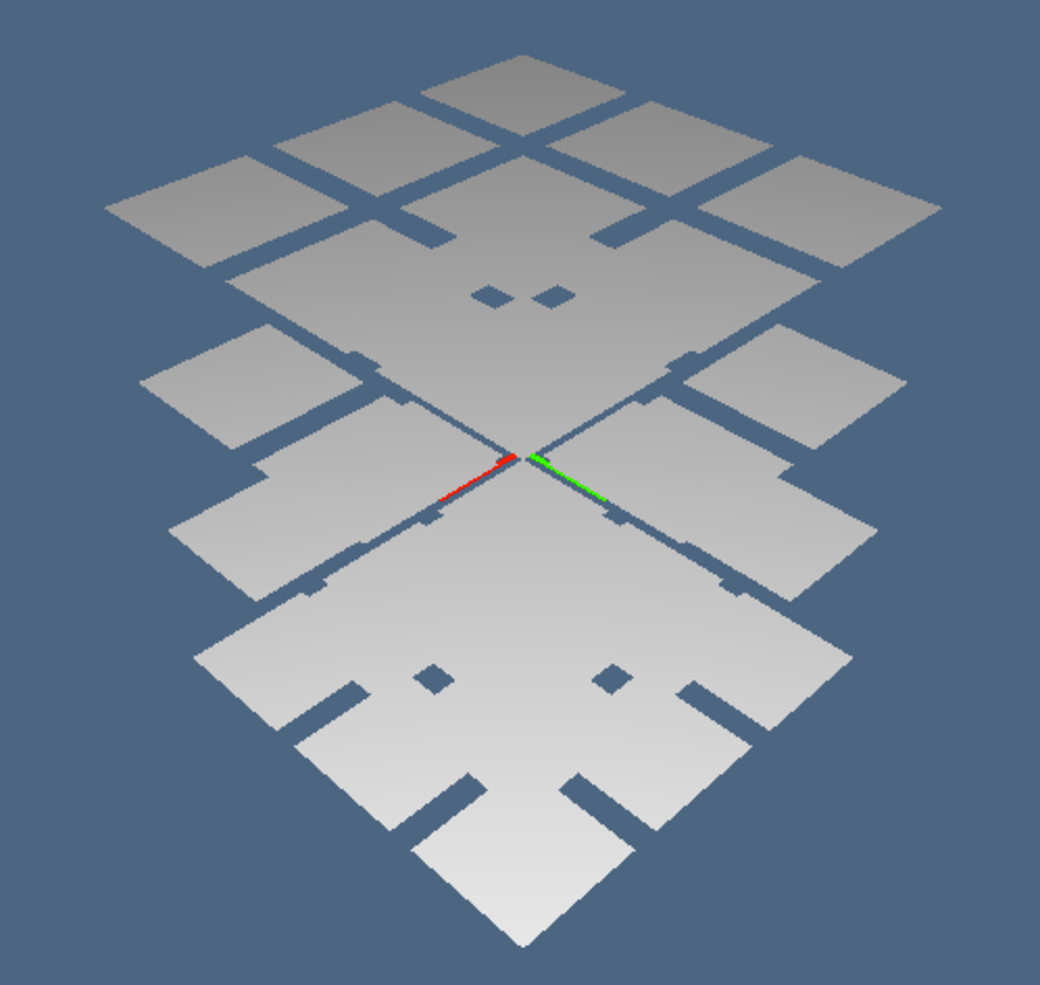
\includegraphics[height=0.245\linewidth,width=0.242\linewidth]{images/skel2c} 
   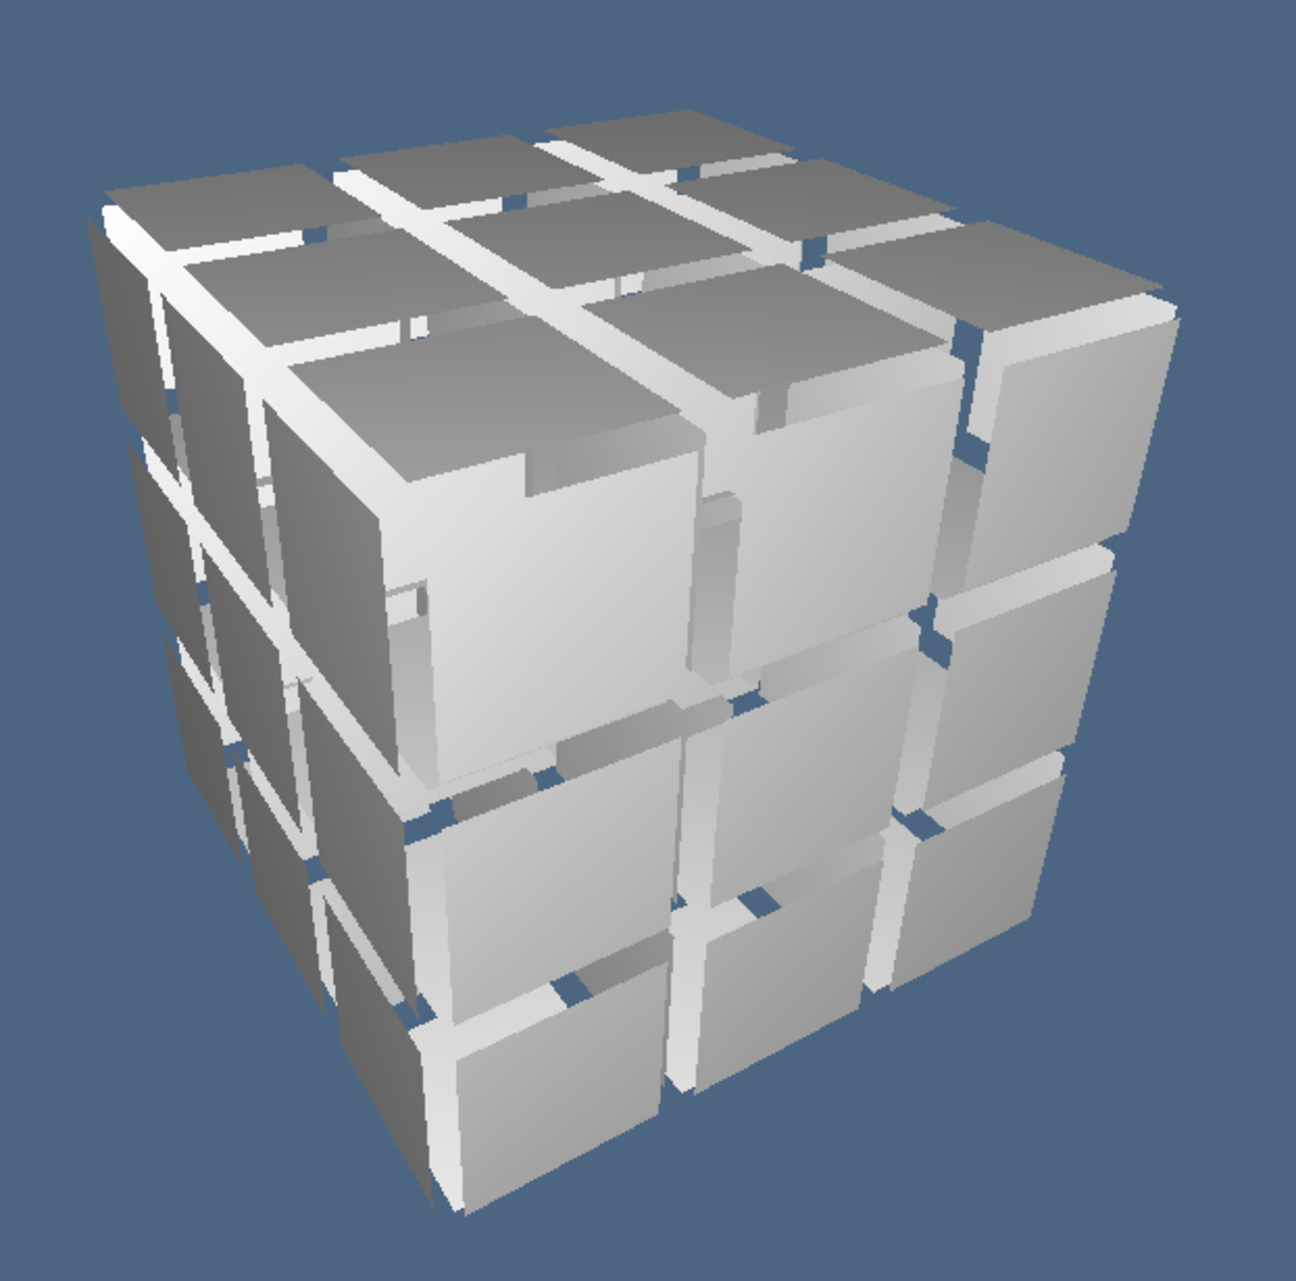
\includegraphics[height=0.245\linewidth,width=0.242\linewidth]{images/skel2} 
   \caption{(a,b,c) Exploded views of subsets (orthogonal to coordinate axes) of 2-cells of a 2-skeleton grid; (d) their assembled set.}
   \label{fig:sleletons}
\end{figure}

%-------------------------------------------------------------------------------
@D Assembling grid skeletons
@{def larGridSkeleton(shape):
    n = len(shape)
    def larGridSkeleton0(d):
        components = filterByOrder(n)[d]
        componentCellLists = [AA(APPLY)(zip( AA(larGrid)(shape),(component) ))
                              for component in components]
        return CAT([ larCellProd(cellLists)  for cellLists in componentCellLists ])
    return larGridSkeleton0
@}
%-------------------------------------------------------------------------------


\begin{figure}[htbp] %  figure placement: here, top, bottom, or page
   \centering
   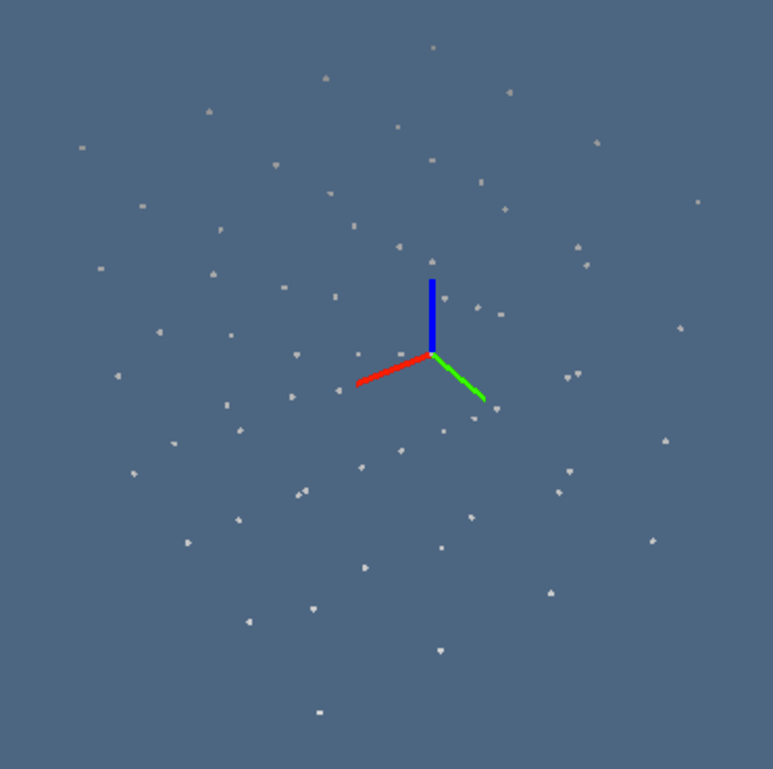
\includegraphics[height=0.245\linewidth,width=0.242\linewidth]{images/skel0} 
   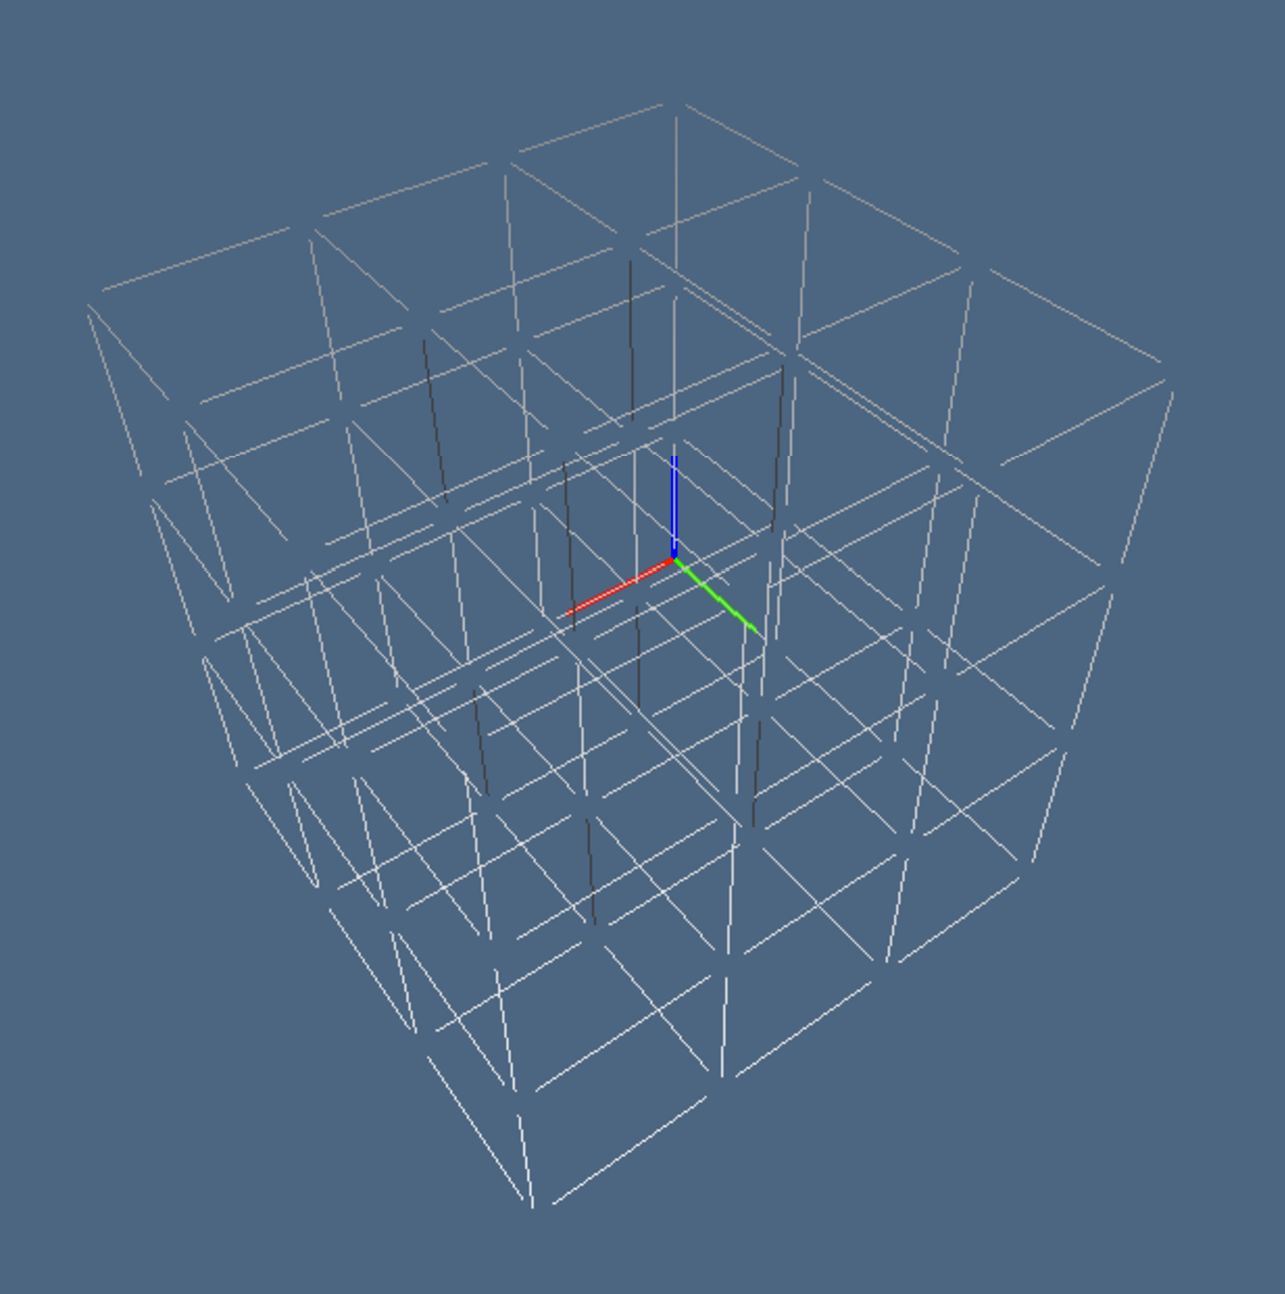
\includegraphics[height=0.245\linewidth,width=0.242\linewidth]{images/skel1} 
   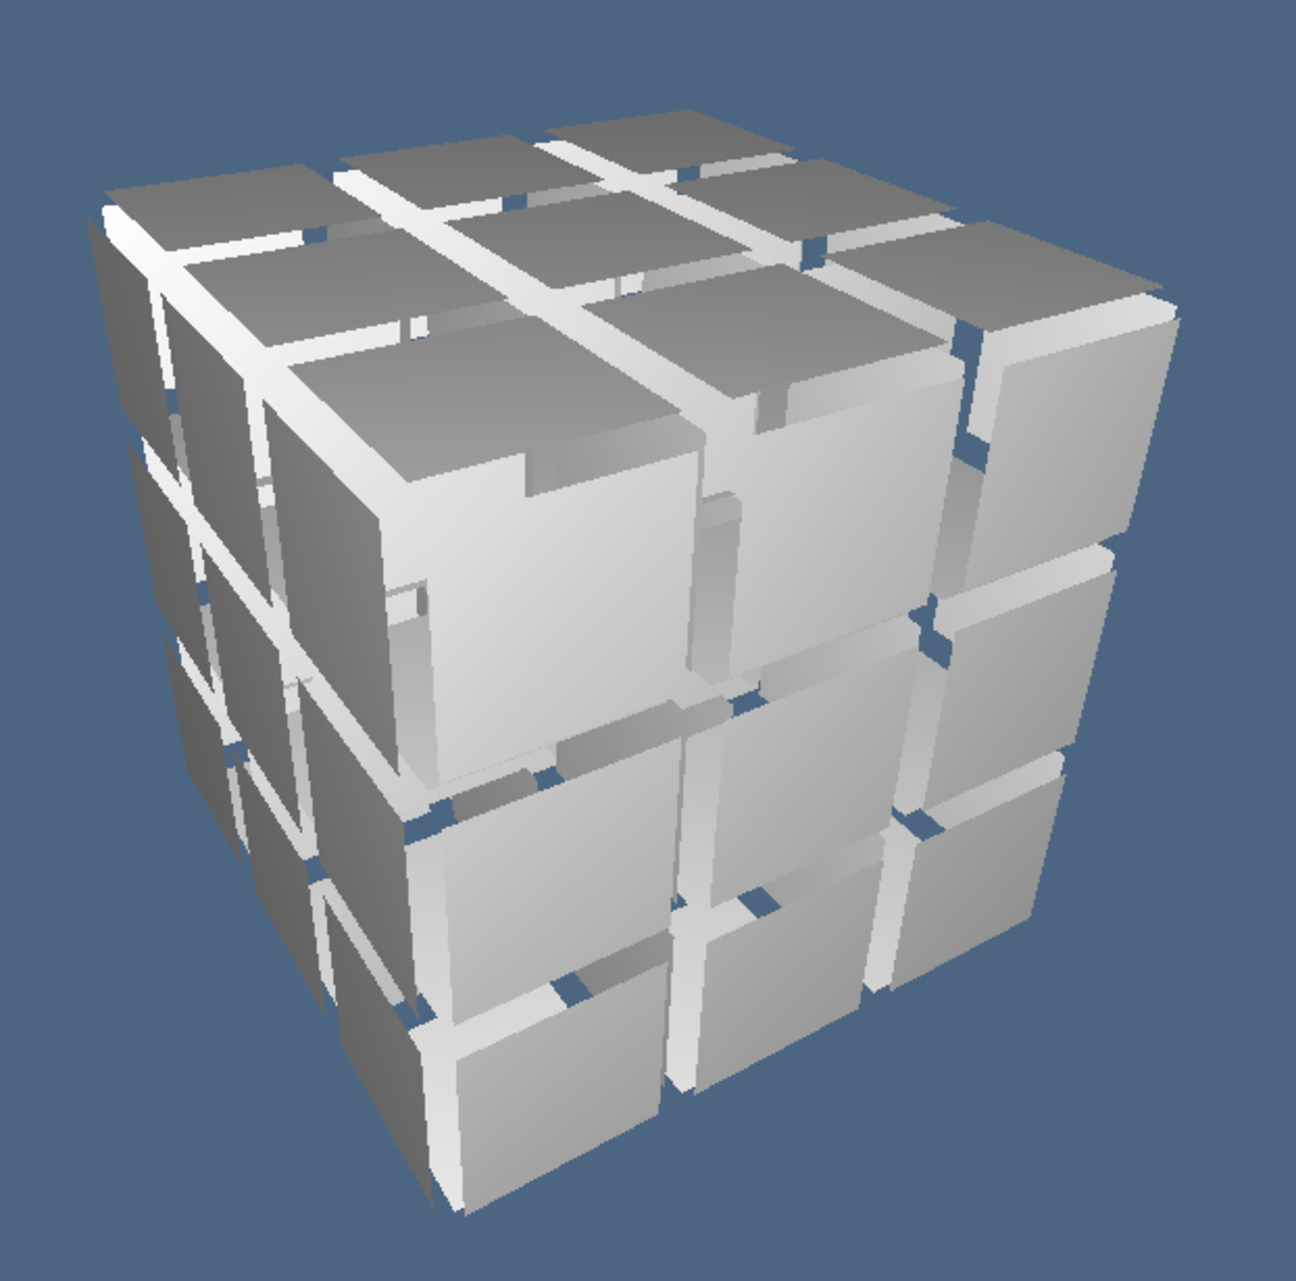
\includegraphics[height=0.245\linewidth,width=0.242\linewidth]{images/skel2} 
   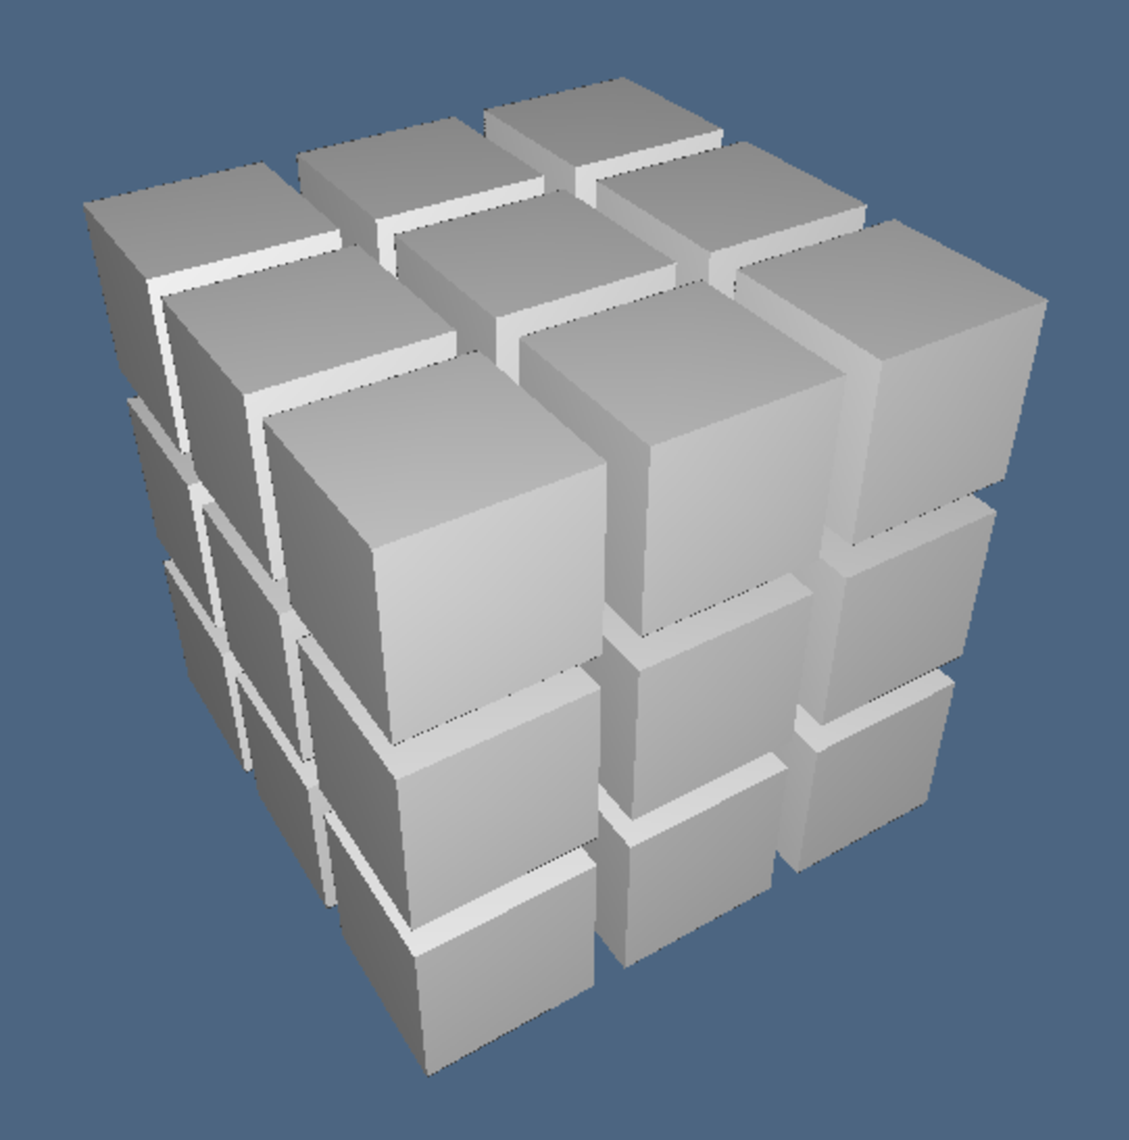
\includegraphics[height=0.245\linewidth,width=0.242\linewidth]{images/skel3} 
   \caption{Exploded views of 0-, 1-, 2-, and 3-dimensional skeletons.}
   \label{fig:grid23D}
\end{figure}

\subsection{Highest-level grid interface}

The highest-level user interface for (hyper)-cuboidal grid generation is given by the function \texttt{larCuboids}  applied to the \texttt{shape} parameter.  
For the sake of storage efficiency, the generated vertex coordinates are integer and 0-based in the lowest corner. The model may be properly scaled and/or translated \emph{a posteriori} when needed.

\paragraph{Generation of (hyper)-cuboidal grids}

The generated complex is always full-dimension, i.e.~\emph{solid}, and possibly includes the cells of all dimensions, depending on the Boolean value of the \texttt{full} parameter.
The grid's intrinsic dimension, as well as the dimension of its embedding space, are specified by the length of the \texttt{shape} parameter. See the examples in Figure~\ref{fig:grid23D}, but remember that the PLaSM visualiser always embed in 3D the displayed model. 

%-------------------------------------------------------------------------------
@D Multidimensional grid generation
@{def larImageVerts(shape):
	def vertexDomain(n): 
		return [[k] for k in range(n)]
	vertLists = [vertexDomain(k+1) for k in shape]
	vertGrid = larVertProd(vertLists)
	return vertGrid

def larCuboids(shape, full=False):
	vertGrid = larImageVerts(shape)
	gridMap = larGridSkeleton(shape)
	if not full: 
		cells = gridMap(len(shape))
	else:
		skeletonIds = range(len(shape)+1)
		cells = [ gridMap(id) for id in skeletonIds ]
	return vertGrid, cells
@}
%-------------------------------------------------------------------------------

\paragraph{Multidimensional visualisation examples}
Visualisation examples of grid of dimension 1,2, and 3 are given below and are displayed  in Figure~\ref{fig:grid23D}. The same input pattern may be used for higher-dimensional grids (say, of dimension 4 and beyond), but to be visualised they should be carefully and properly projected in 3D.

%-------------------------------------------------------------------------------
@d Multidimensional visualisation examples
@{def mergeSkeletons(larSkeletons): return larSkeletons[0],CAT(larSkeletons[1])
VIEW(EXPLODE(1.5,1.5,1.5)(MKPOLS(mergeSkeletons(larCuboids([3],True)))))
VIEW(EXPLODE(1.5,1.5,1.5)(MKPOLS(mergeSkeletons(larCuboids([3,2],True)))))
VIEW(EXPLODE(1.5,1.5,1.5)(MKPOLS(mergeSkeletons(larCuboids([3,2,1],True)))))
@}
%-------------------------------------------------------------------------------

\begin{figure}[htbp] %  figure placement: here, top, bottom, or page
   \centering
   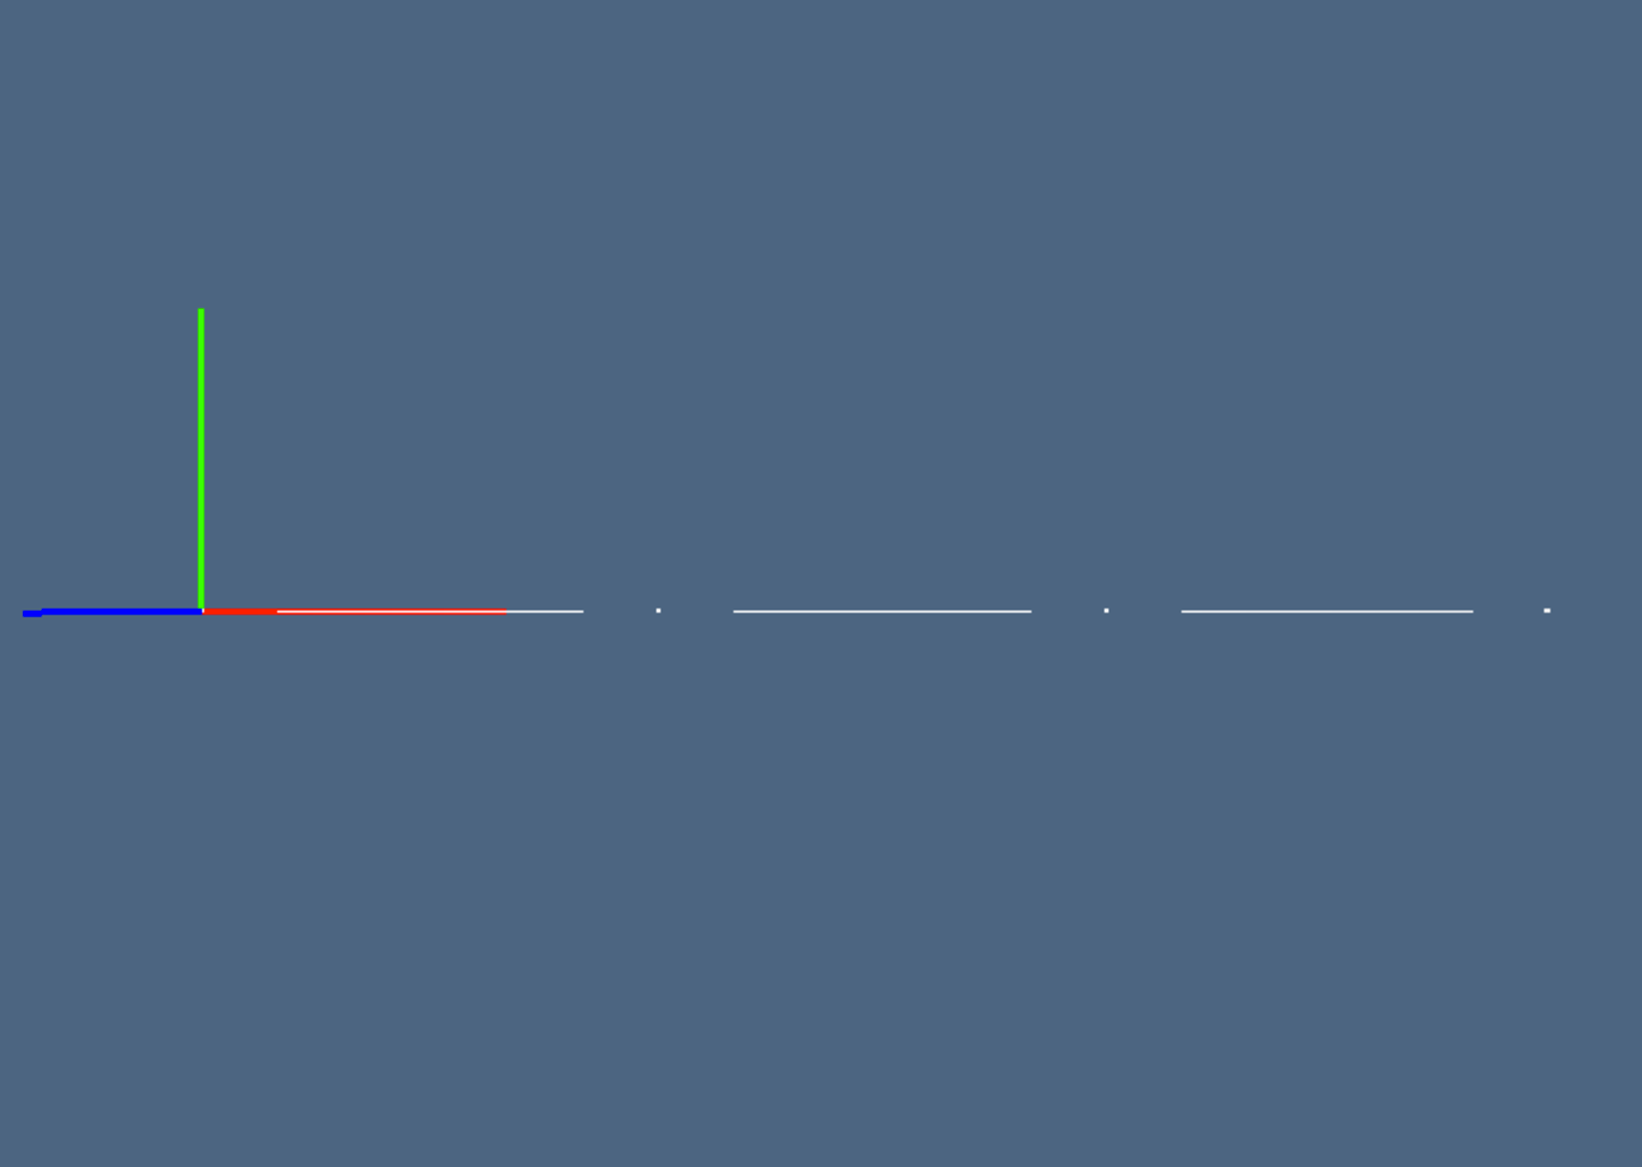
\includegraphics[width=0.313\linewidth]{images/complex3} 
   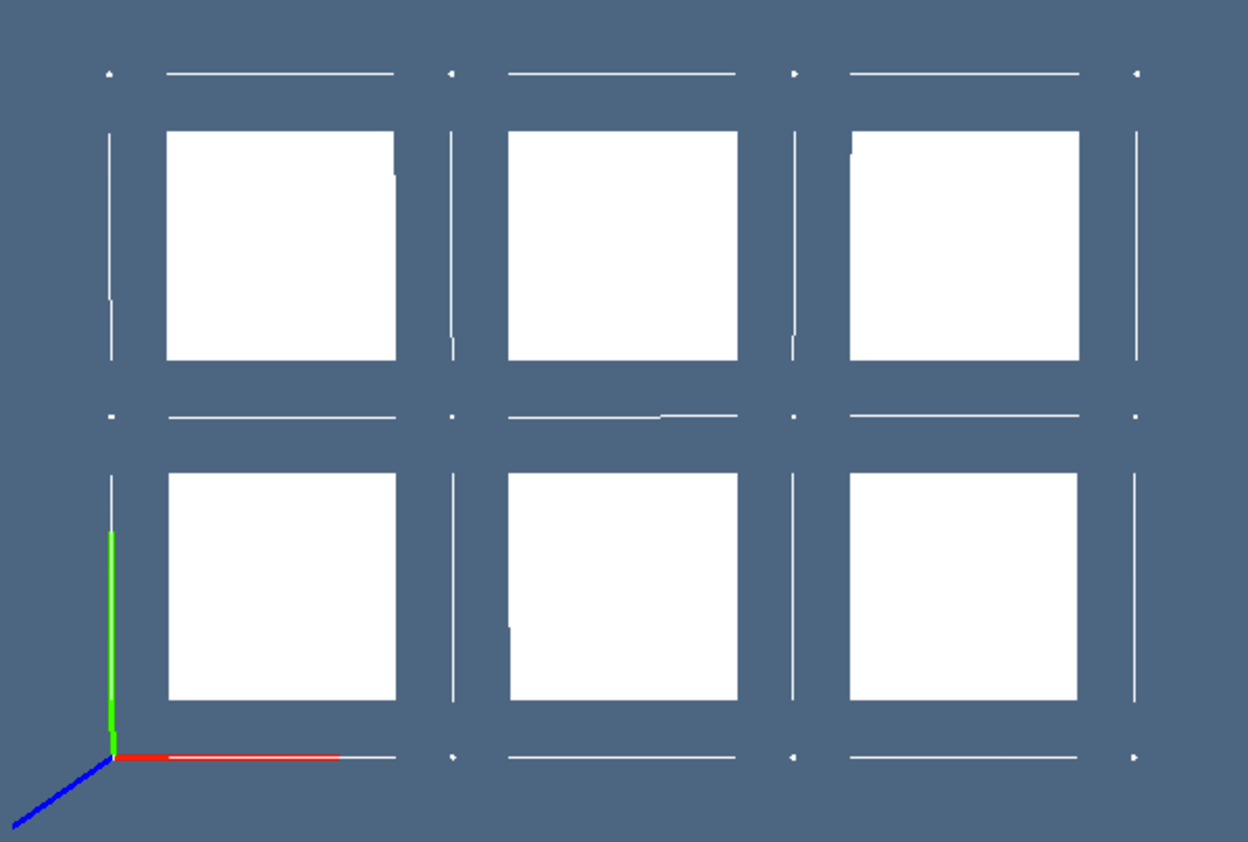
\includegraphics[width=0.33\linewidth]{images/complex32} 
   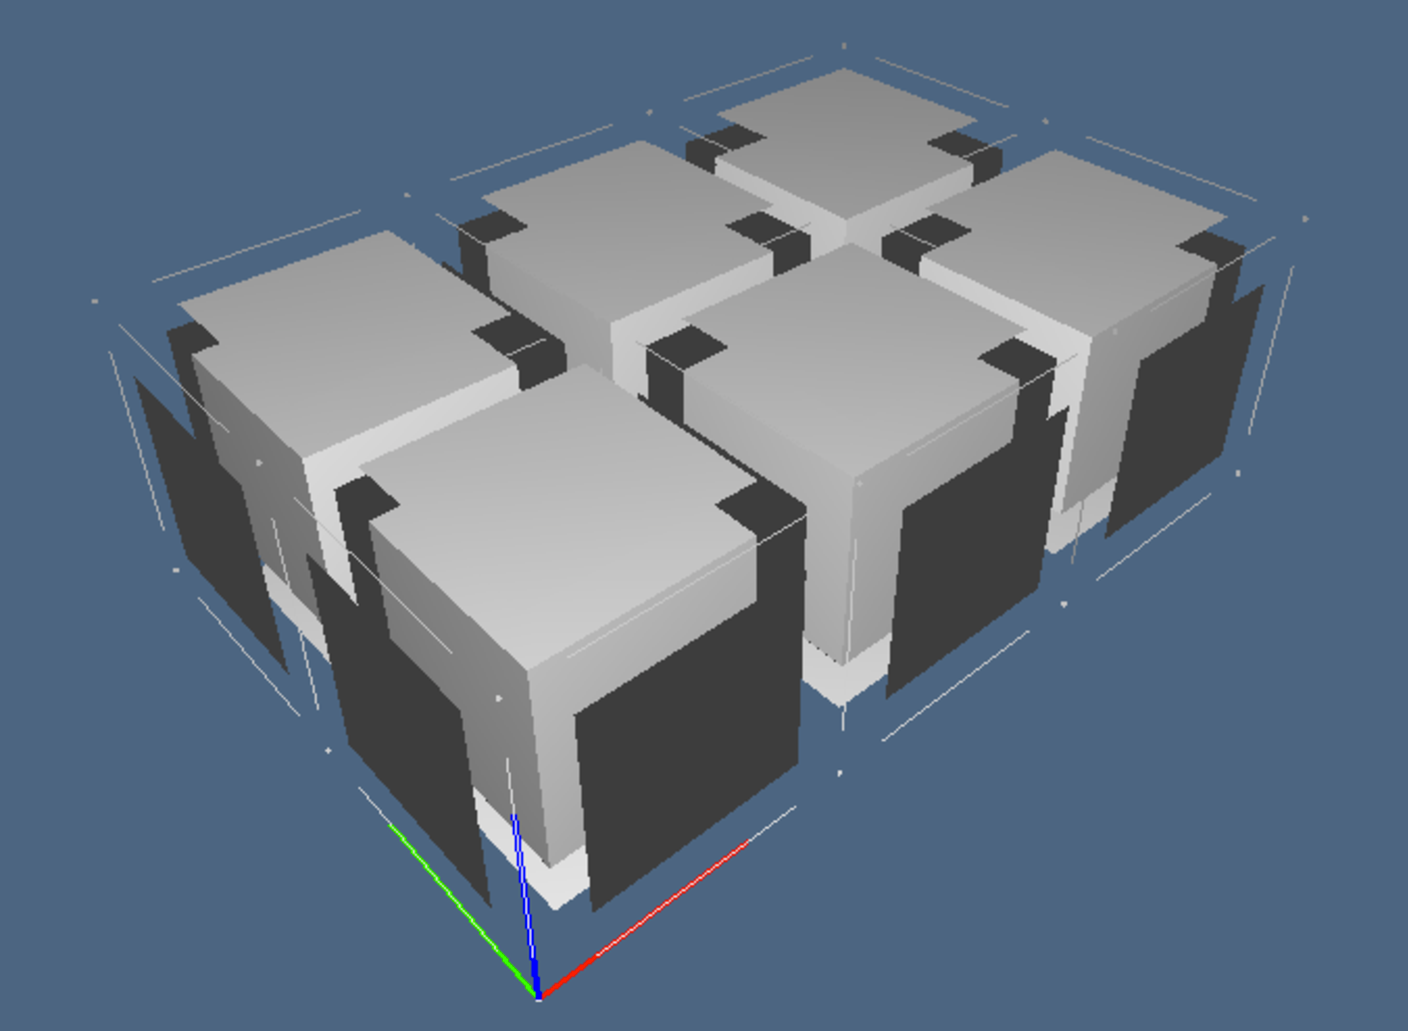
\includegraphics[width=0.305\linewidth]{images/complex321} 
   \caption{Exploded views of 1D, 2D, and 3D cellular complexes (including cells of dimension 0,1,2, and 3).}
   \label{fig:grid23D}
\end{figure}


\subsection{Chain of boundary operators}

As we know, a \emph{chain complex} is a sequence of (linear) chain spaces $C_k$ ($d\geq k\geq 0$) and a sequence
of boundary operators $\partial_k: C_k \to C_{k-1}$ ($d\geq k\geq 1$) between adjacent spaces (see Figure~\ref{fig:chainComplexMap}). In this section, we aim to generate the sequence of boundary matrices \texttt{CSR($[\partial_k]$)} ($1\leq k\leq d$).

\begin{figure}[htbp] %  figure placement: here, top, bottom, or page
   \centering
   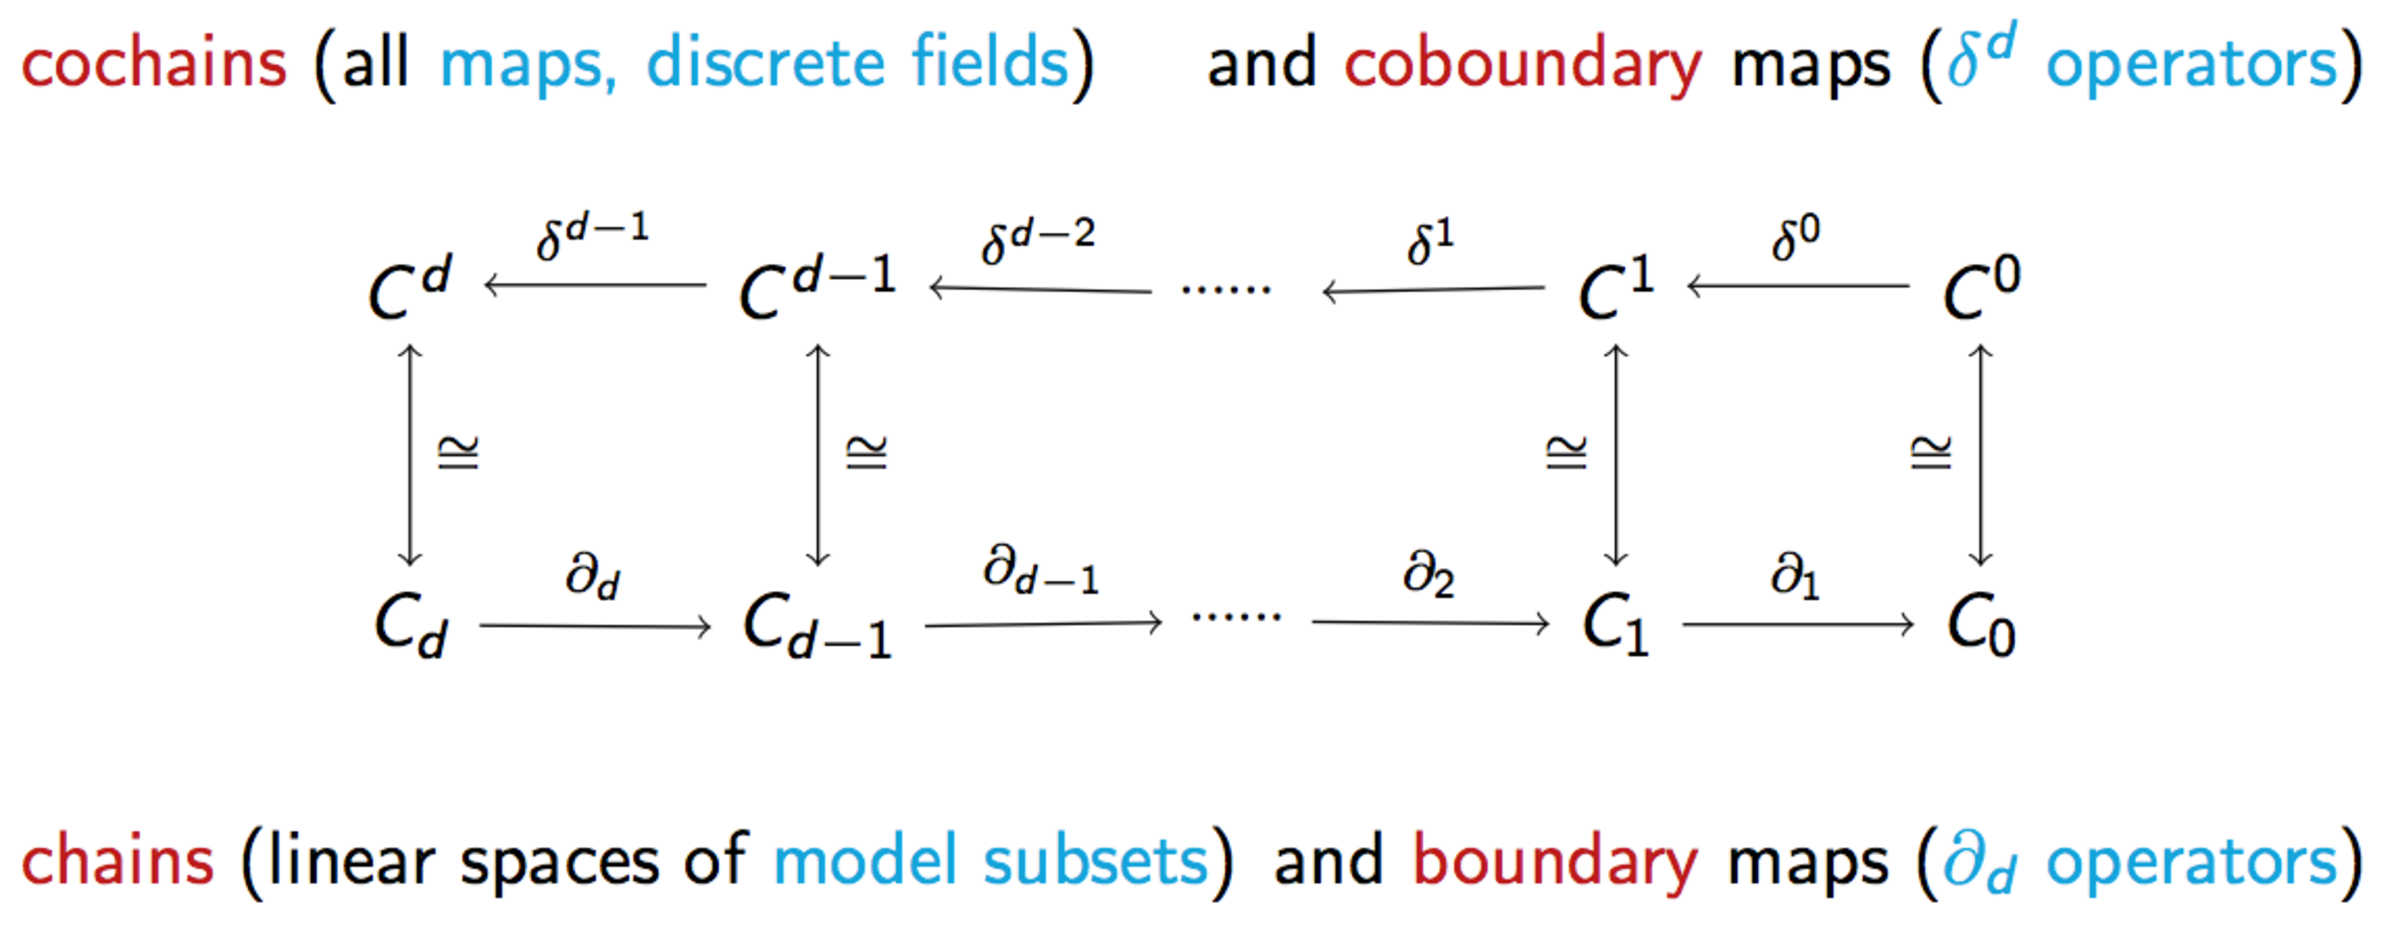
\includegraphics[width=0.8\linewidth]{images/chainComplexMap} 
   \caption{Chain and cochain complexes.}
   \label{fig:chainComplexMap}
\end{figure}

\paragraph{Cuboidal skeletons}
A list of \texttt{BRC} characteristic matrices of cellular $k$-complexes ($0\leq k\leq d$) with dimension $d$, where $d={}$\texttt{len(shape)}, is returned by the function \texttt{gridSkeletons} in the macro below, where the input is given by the \emph{shape} of the grid, i.e.~by the list of cell items in each coordinate direction. Some simple test examples of skeletons of cuboidal complexes are also printed when the \texttt{largrid} module run as the \texttt{main}. Just notice that the number of returned $d$-cells is equal to \texttt{PROD(shape)}.

%-------------------------------------------------------------------------------
@D Multidimensional grid skeletons
@{def gridSkeletons(shape):
	gridMap = larGridSkeleton(shape)
	skeletonIds = range(len(shape)+1)
	skeletons = [ gridMap(id) for id in skeletonIds ]
	return skeletons
	
if __name__=="__main__":
	print "\ngridSkeletons([3]) =\n", gridSkeletons([3])
	print "\ngridSkeletons([3,2]) =\n", gridSkeletons([3,2])
	print "\ngridSkeletons([3,2,1]) =\n", gridSkeletons([3,2,1])
@}
%-------------------------------------------------------------------------------

\paragraph{Boundary complex of a cuboidal grid}
The list of boundary matrices \texttt{CSR($[\partial_k]$)} ($1\leq k\leq d$) is returned by the function
\texttt{gridBoundaryMatrices}.

%-------------------------------------------------------------------------------
@D Generation of grid boundary complex
@{def gridBoundaryMatrices(shape):
	skeletons = gridSkeletons(shape)
	boundaryMatrices = [boundary(skeletons[k+1],faces) 
						 for k,faces in enumerate(skeletons[:-1])]
	return boundaryMatrices
	
if __name__=="__main__":
	for k in range(1):
		print "\ngridBoundaryMatrices([3]) =\n", \
				csr2DenseMatrix(gridBoundaryMatrices([3])[k])
	for k in range(2):
		print "\ngridBoundaryMatrices([3,2]) =\n", \
				csr2DenseMatrix(gridBoundaryMatrices([3,2])[k])
	for k in range(3):
		print "\ngridBoundaryMatrices([3,2,1]) =\n", \
				csr2DenseMatrix(gridBoundaryMatrices([3,2,1])[k])
@}
%-------------------------------------------------------------------------------

%===============================================================================
\section{Face stack of cellular complexes}
\label{sec:facestack}
%===============================================================================

%-------------------------------------------------------------------------------
\subsection{Simplicial complexes}
%-------------------------------------------------------------------------------

The stack of faces of a simplicial $d$-complex is easy to compute making use of the combinatorial properties of the simplex boundary. If the input is the compressed sparse row representation \texttt{CSR}$(M_d)$ of the binary characteristic matrix $M_d$ of the highest rank cells ($d$-simplices), we repeatedly apply the \texttt{larSimplexFacets} function.

\paragraph{Simplicial face stack computation}
The whole stack of \texttt{LAR} cell-vertex arrays is computed below for the multidimensional case, and returned ordered from 0-cells to $d$-cells.

%-------------------------------------------------------------------------------
@D Simplicial face stack computation
@{""" Simplicial face stack computation """
def larSimplicialStack(simplices):
	dim = len(simplices[0])-1
	faceStack = [simplices]
	for k in range(dim):
		faces = larSimplexFacets(faceStack[-1])
		faceStack.append(faces)
	return REVERSE(faceStack)
@}
%-------------------------------------------------------------------------------

\paragraph{Oriented boundary: Example 2D}
The file \texttt{test/py/largrid/test04.py} gives an example of computation of the oriented 1D boundary of a 2D simplicial grid. In the variable \texttt{bases} we store the stack of bases of $k$-chains, for $0\leq k\leq 2$. The variable \texttt{boundaryCells} contains the indices of boundary cells, signed according to their absolute orientation. To get a coherent orientation of the model boundary, the boundary 2-cells with negative indices must undergo to reversing their orientation.
 
%-------------------------------------------------------------------------------
@O test/py/largrid/test04.py
@{""" Computation of the boundary of a simplicial grid """
import sys; sys.path.insert(0, 'lib/py/')
from larcc import *
from largrid import *

V,simplices = larSimplexGrid1((2,2))
bases = larSimplicialStack(simplices)
boundaryCells = signedBoundaryCells(V,bases[-1],bases[-2])

def swap(mylist): return [mylist[1]]+[mylist[0]]+mylist[2:]
orientedBoundary = [bases[-2][-k] if k<0 else swap(bases[-2][k]) 
						for k in boundaryCells]
VIEW(EXPLODE(1.2,1.2,1.2)(MKPOLS((V,orientedBoundary))))
submodel = STRUCT(MKPOLS((V,orientedBoundary)))
VIEW(larModelNumbering(V,bases,submodel))
@}
%-------------------------------------------------------------------------------


\paragraph{Oriented boundary: Example 3D}
A very similar example is given below for a 3D simplicial grid, in order to show 
how to use the components of the LAR cell stack, computed as \texttt{larSimplicialStack(CV)}, and stored in the \texttt{bases} variable. T

%-------------------------------------------------------------------------------
@O test/py/largrid/test03.py
@{""" Computation of the boundary of a simplicial grid """
import sys; sys.path.insert(0, 'lib/py/')
from larcc import *
from largrid import *

V,CV = larSimplexGrid1((2,2,2))
bases = larSimplicialStack(CV)
VV,EV,FV,CV = bases
boundaryCells = signedBoundaryCells(V,CV,FV)

def swap(mylist): return [mylist[1]]+[mylist[0]]+mylist[2:]
orientedBoundary = [FV[-k] if k<0 else swap(FV[k]) for k in boundaryCells]
VIEW(EXPLODE(1.2,1.2,1.2)(MKPOLS((V,orientedBoundary))))
submodel = EXPLODE(1.05,1.05,1.05)(MKPOLS((V,orientedBoundary)))
VIEW(larModelNumbering(V,bases,submodel))
@}
%-------------------------------------------------------------------------------

%-------------------------------------------------------------------------------
\subsection{Cuboidal complexes}
%-------------------------------------------------------------------------------


\paragraph{Example 2D}

%-------------------------------------------------------------------------------
@O test/py/largrid/test05.py
@{""" Extraction of oriented boundary of a cuboidal 2-complex """
import sys; sys.path.insert(0, 'lib/py/')
from largrid import *
from random import random

shape = 20,20
V,cells = larCuboids(shape)
cellSpan = prod(shape)
fraction = 0.9
remove = [int(random()*cellSpan) for k in range(int(cellSpan*fraction)) ]
cells = [cells[k] for k in range(cellSpan) if not k in remove]
V,EV = larCuboidsFacets((V,cells))
VIEW(EXPLODE(1.2,1.2,1)(MKPOLS((V,EV))))

boundaryCells = signedBoundaryCells(V,cells,EV)
def swap(mylist): return [mylist[1]]+[mylist[0]]+mylist[2:]
orientedBoundary = [EV[-k] if k<0 else swap(EV[k]) for k in boundaryCells]
VIEW(EXPLODE(1.2,1.2,1.2)(MKPOLS((V,orientedBoundary))))

@}
%-------------------------------------------------------------------------------


\begin{figure}[htbp] %  figure placement: here, top, bottom, or page
   \centering
   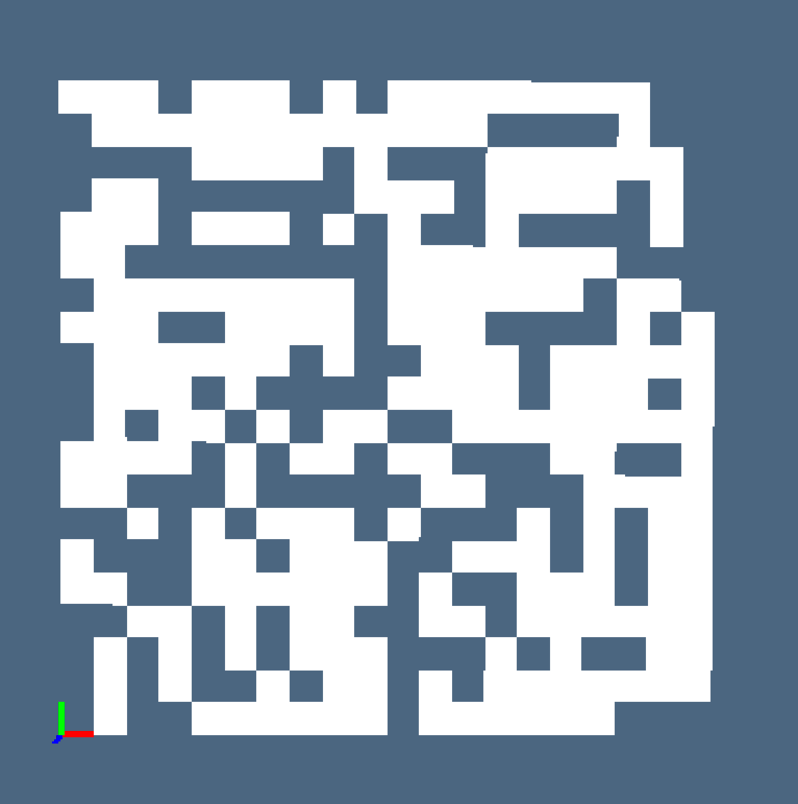
\includegraphics[height=0.245\linewidth,width=0.244\linewidth]{images/2Dsigned0} 
   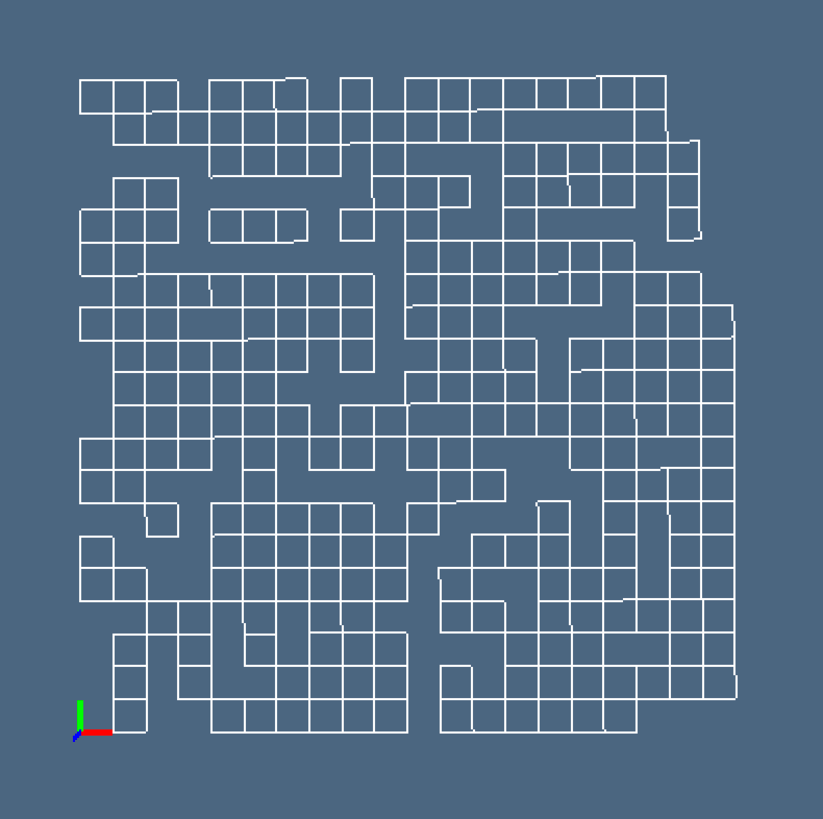
\includegraphics[height=0.245\linewidth,width=0.244\linewidth]{images/2Dsigned1} 
   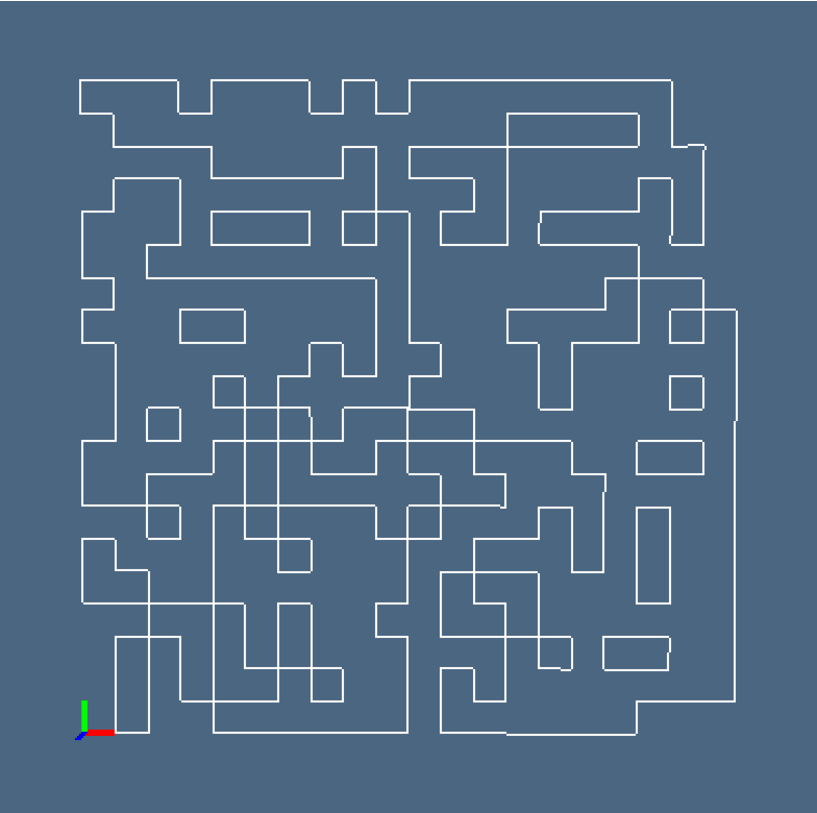
\includegraphics[height=0.245\linewidth,width=0.244\linewidth]{images/2Dsigned2} 
   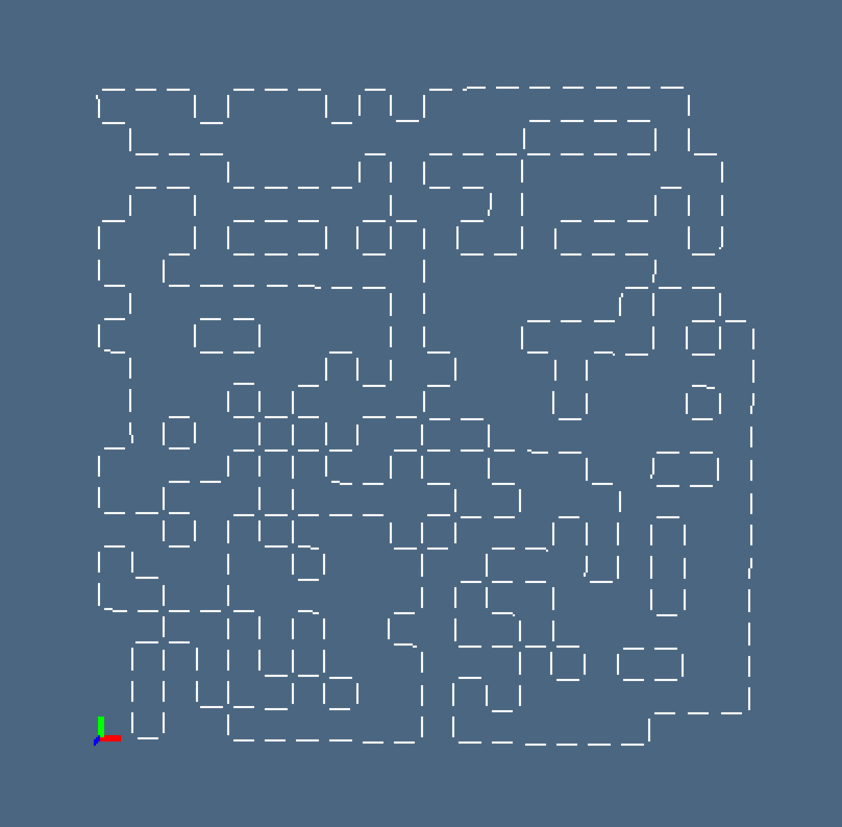
\includegraphics[height=0.245\linewidth,width=0.244\linewidth]{images/2Dsigned3} 
   \caption{Extraction of oriented boundary of a cuboidal 2-complex: (a) The cellular 2-complex; (b) complex of 1-cells; (c) oriented boundary; (d) exploded boundary.}
	\vspace{3mm}
   \centering
   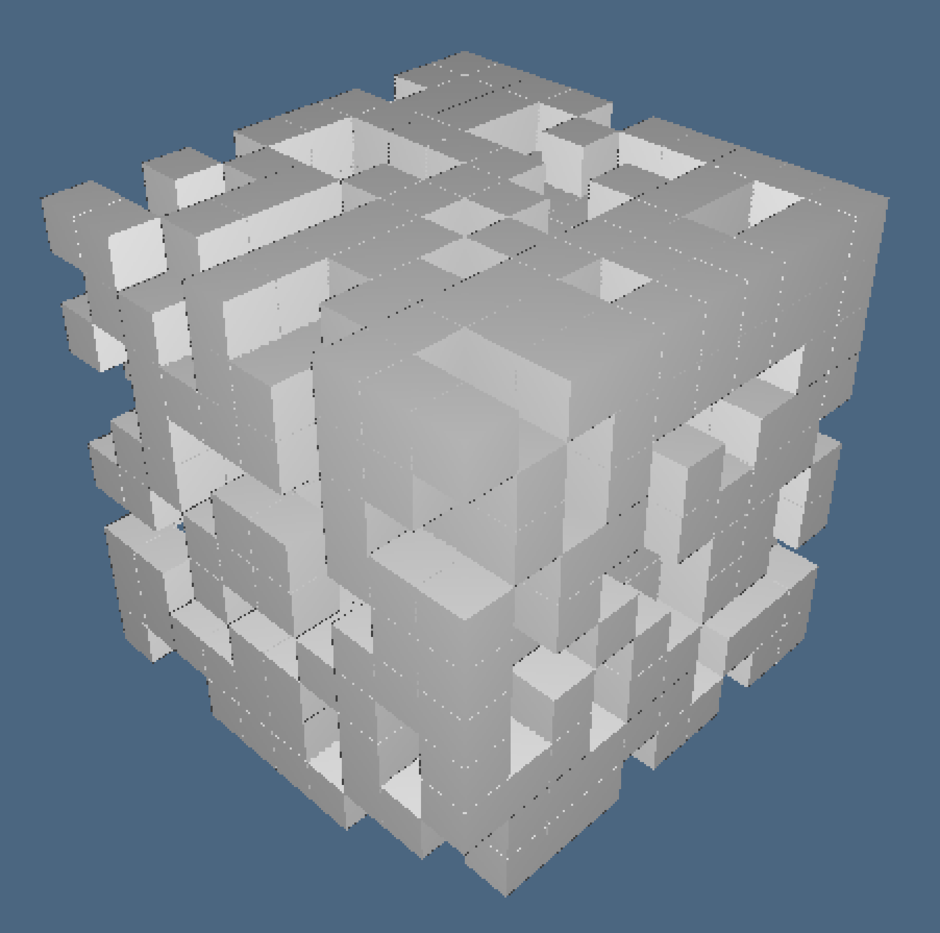
\includegraphics[height=0.245\linewidth,width=0.244\linewidth]{images/3Dsigned0} 
   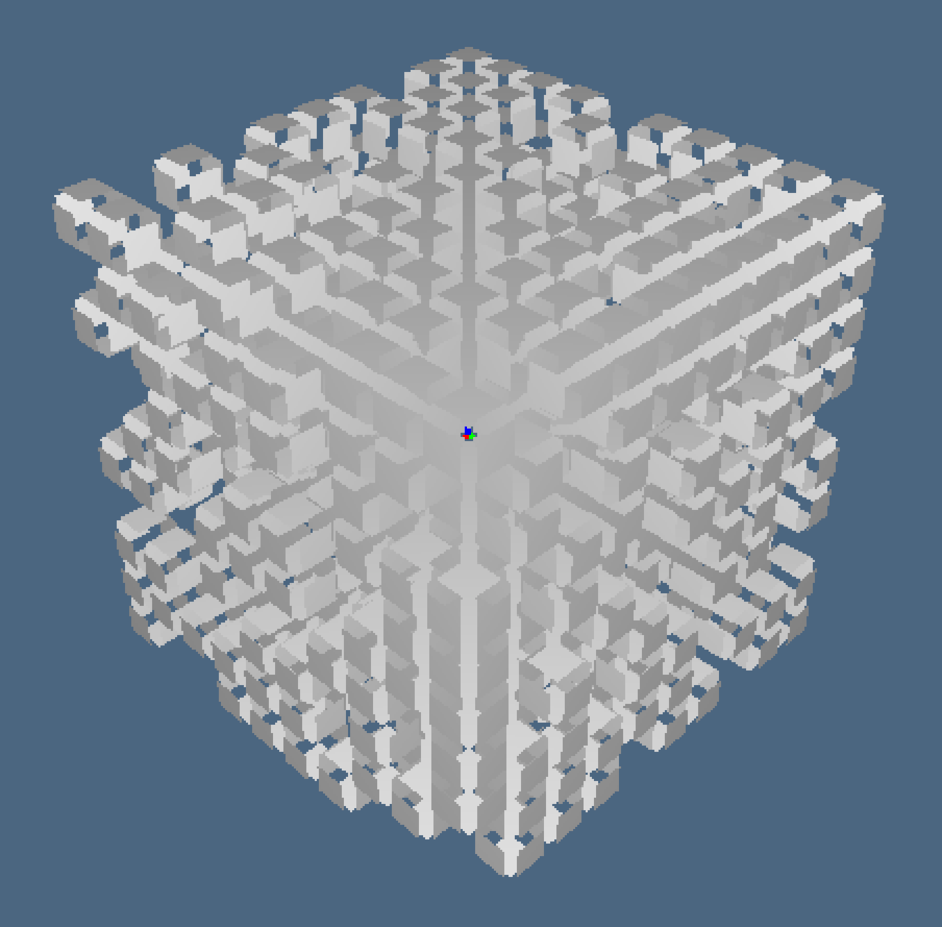
\includegraphics[height=0.245\linewidth,width=0.244\linewidth]{images/3Dsigned1} 
   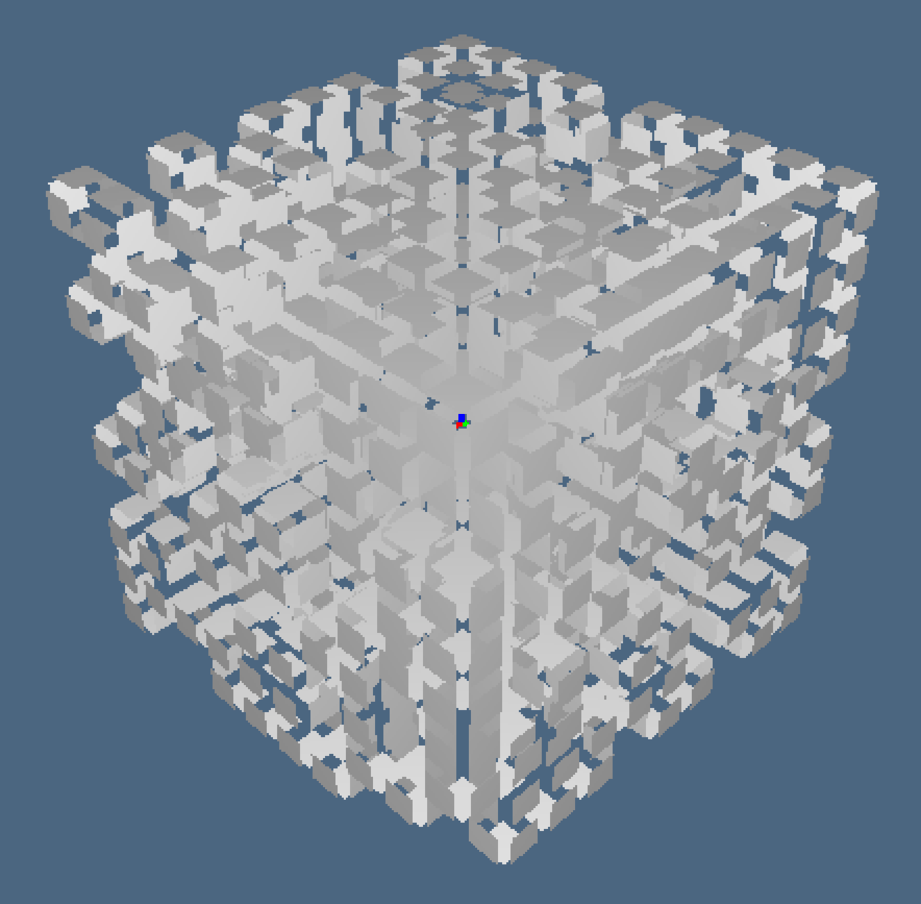
\includegraphics[height=0.245\linewidth,width=0.244\linewidth]{images/3Dsigned2} 
   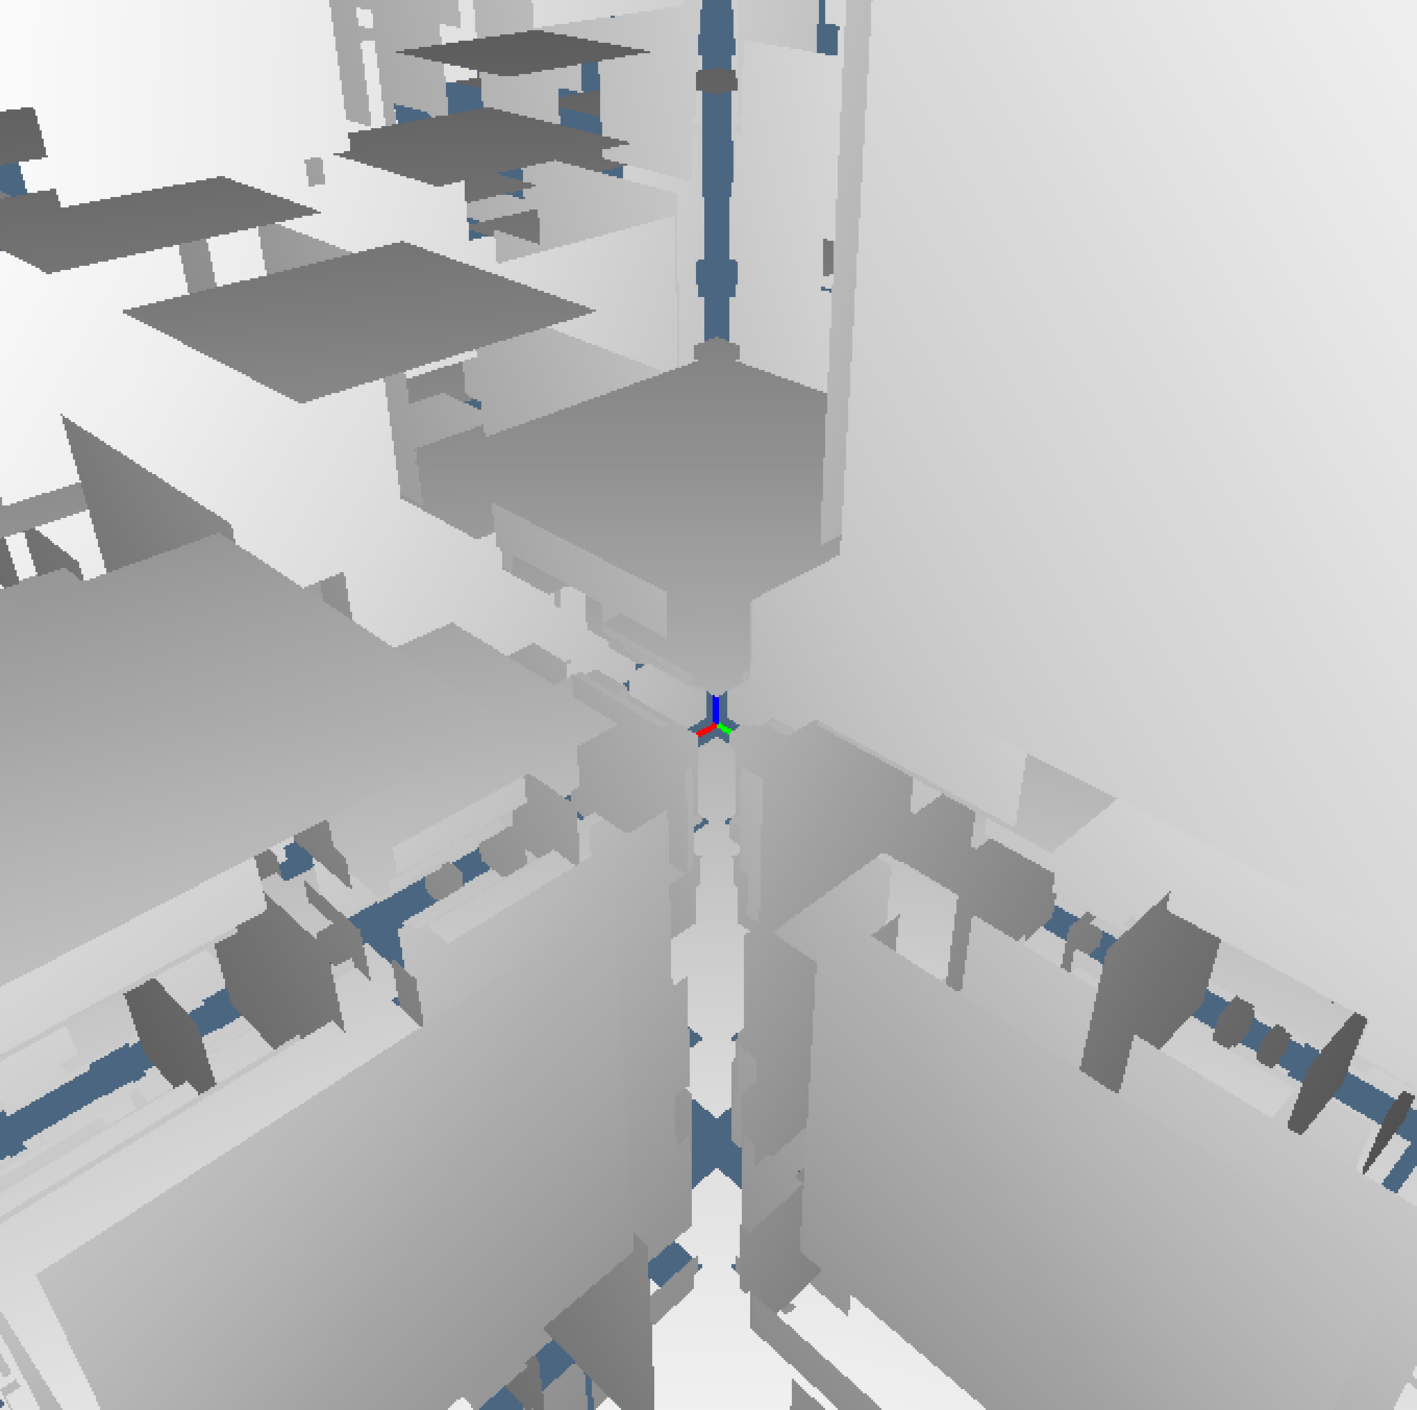
\includegraphics[height=0.245\linewidth,width=0.244\linewidth]{images/3Dsigned3} 
   \caption{Extraction of oriented boundary of a cuboidal 3-complex: (a) Cellular 3-complex; (b) complex of 2-cells; (c) (exploded) oriented boundary; (d) view from the boundary interior.}
   \label{fig:2-3-complex}
\end{figure}


\paragraph{Example 3D}

%-------------------------------------------------------------------------------
@O test/py/largrid/test06.py
@{""" Extraction of oriented boundary of a cuboidal 3-complex """
import sys; sys.path.insert(0, 'lib/py/')
from largrid import *
from random import random

shape = (10,10,10)
V,cells = larCuboids(shape)
cellSpan = prod(shape)
fraction = 0.9
remove = [int(random()*cellSpan) for k in range(int(cellSpan*fraction)) ]
cells = [cells[k] for k in range(cellSpan) if not k in remove]
V,FV = larCuboidsFacets((V,cells))
VIEW(EXPLODE(1.2,1.2,1.2)(MKPOLS((V,FV))))
@}
%-------------------------------------------------------------------------------



\subsubsection{Random polytopal complexes}


\paragraph{Extraction of facets from cuboidal complexes}

%-------------------------------------------------------------------------------
@D Extraction of facets from cuboidal complexes
@{""" Extraction of facets from cuboidal complexes """
def larCuboidsFacets((V,cells)):
	dim = len(V[0])
	n = int(2**(dim-1))
	facets = []
	for cell in cells:
		coords = [AR([V[v],v]) for v in cell] # decorate coords with vertex index
		doubleFacets = [sorted(coords,key=(lambda x: x[k])) for k in range(dim)]
		facets += AA(AA(LAST))(CAT([[pair[:n],pair[n:]] for pair in doubleFacets]))
	facets = AA(eval)(set(AA(str)(facets))) # remove duplicates
	return V,sorted(facets)

if __name__ == "__main__":
	VIEW(EXPLODE(1.2,1.2,1.2)(MKPOLS(larCuboidsFacets(larCuboids([3,3,3])))))
@}
%-------------------------------------------------------------------------------


%-------------------------------------------------------------------------------
\subsection{Polytopal complexes}
%-------------------------------------------------------------------------------

TODO

%-------------------------------------------------------------------------------
%===============================================================================
\section{Cartesian product of cellular complexes}
\label{sec:product}
%===============================================================================

\paragraph{LAR model of cellular complexes}

The external representation of a LAR model (necessarily geometrical, i.e.~embedded in some $\E^n$, in order to be possible to draw it) is a pair (\emph{geometry},\emph{topology}), where \emph{geometry} is the list of coordinates of vertices, i.e.~a two-dimensional array of numbers, where vertices are given by row, and \emph{topology} is a list of cells of fixed dimension $d$. When $d=n$ the model is \emph{solid}; otherwise  the model is some emberdded $d$-skeleton ($0\leq d <n$).

\paragraph{Binary product of cellular complexes}
The \texttt{larModelProduct} function takes as input a pair of LAR models and returns the model of their Cartesian product. Since this is a pair (\emph{geometry}, \emph{topology}), its second element returns the topological product of the input topologies.

%-------------------------------------------------------------------------------
@d Cartesian product of two lar models  
@{def larModelProduct(twoModels):
    (V, cells1), (W, cells2) = twoModels
    @< Cartesian product of vertices @>
    @< Topological product of cells    @>
    model = [list(v) for v in vertices.keys()], cells
    return model
@}
%-------------------------------------------------------------------------------

\paragraph{Cartesian product of argument vertices}
The following macro is used to generate a dictionary mapping between integer ids of new vertices and the sets $V$ and $W$ of vertices of the input complexes.

%-------------------------------------------------------------------------------
@d Cartesian product of vertices  
@{vertices = collections.OrderedDict(); k = 0
for v in V:
    for w in W:
        id = tuple(v+w)
        if not vertices.has_key(id):
            vertices[id] = k
            k += 1	@}
%-------------------------------------------------------------------------------


\paragraph{Topological product of argument vertices}
Another macro generates the cells of the topological product, represented as lists of new vertices. 

%-------------------------------------------------------------------------------
@d Topological product of cells    
@{cells = [ [vertices[tuple(V[v] + W[w])] for v in c1 for w in c2]
         for c1 in cells1 for c2 in cells2]	@}
%-------------------------------------------------------------------------------


%-------------------------------------------------------------------------------
@d Test examples of Cartesian product
@{if __name__ == "__main__":
    geom_0,topol_0 = [[0.],[1.],[2.],[3.],[4.]],[[0,1],[1,2],[2,3],[3,4]]
    geom_1,topol_1 = [[0.],[1.],[2.]], [[0,1],[1,2]]
    mod_0 = (geom_0,topol_0)
    mod_1 = (geom_1,topol_1)
    squares = larModelProduct([mod_0,mod_1])
    VIEW(EXPLODE(1.2,1.2,1.2)(MKPOLS(squares)))
    cubes = larModelProduct([squares,mod_0])
    VIEW(EXPLODE(1.2,1.2,1.2)(MKPOLS(cubes)))
@}
%-------------------------------------------------------------------------------



\section{Largrid exporting}
\label{sec:largrid}
In this section we assemble top-down the \texttt{largrid} module, by orderly listing the macros it is composed of. As might be expected, the present one is the module version corresponding to the current state of the system, i.e.~to a very initial state. Other functions will be added when needed, and the module translation in different languages (C/C++, Javascript, Haskell, OpenCL kernels) will be (hopefully soon) appended.
%------------------------------------------------------------------
@O lib/py/largrid.py
@{"""Module with functions for grid generation and Cartesian product"""
import collections
@< Importing \texttt{simplexn} and \texttt{numpy} libraries @>
@< Import the module @(larcc@) @>
@< Generation of vertices of decompositions of 1D intervals  @>
@< Generation of uniform 0D cellular complex  @>
@< Generation of uniform 1D cellular complex  @>
@< Generation of cellular complex of 0/1 dimension $d$ @>
@< Generation of grid vertices  @>
@< Transformation from multindex to address in a linear array storage @>
@< Generation of grid cells  @>
@< Enumeration of binary ranges of given order @>
@< Filtering binary ranges by order @>
@< Assembling grid skeletons @>
@< Multidimensional grid generation @>
@< Multidimensional grid skeletons @>
@< Generation of grid boundary complex @>
@< Cartesian product of two lar models   @>
@< Simplicial face stack computation @>
@< Extraction of facets from cuboidal complexes @>
if __name__=="__main__":
	@< Multidimensional visualisation examples @>
	@< Test examples of Cartesian product @>
@}
%------------------------------------------------------------------


\section{Unit tests}
\label{sec:tests}

\subsection{Creation of repository of unit tests}

A possible unit test strategy is to create a directory for unit tests associated to each source file in \texttt{nuweb}. Therefore we create here a directory in \texttt{test/py/} with the same name of the present document. Of course other 

%------------------------------------------------------------------
@d Create directory and echo of creation
@{@< Create directory from path @>
@%i lib/py/largrid
createDir('@1')
print "'@1' repository created"
@}
%------------------------------------------------------------------

%------------------------------------------------------------------
@o test/py/largrid/test01.py
@{@< Create directory  and echo of creation: @(test/py/largrid/@) @>
@}
%------------------------------------------------------------------


\paragraph{Vertices of 1D decompositions}
Some test examples of the \texttt{larSplit} function are given in the following. First the unit interval $[0,1]$ is splitter into 10 sub intervals, then the $[0,2\pi]$ interval is split into 12 parts, used to generate a polyonal approximatetion of the unit circle $S_1$, centred in the origin and with unit radius.

%-------------------------------------------------------------------------------
@O test/py/largrid/test01.py
@{from pyplasm import *

@<Generation of vertices of decompositions of 1D intervals@>
assert larSplit(1)(3) == [[0.0], [0.3333333333333333], [0.6666666666666666], [1.0]]
assert larSplit(1)(1) == [[0.0], [1.0]]
assert larSplit(2*PI)(12) == [[0.0], [0.5235987755982988], [1.0471975511965976], 
[1.5707963267948966], [2.0943951023931953], [2.617993877991494], 
[3.141592653589793], [3.665191429188092], [4.1887902047863905], 
[4.71238898038469], [5.235987755982988], [5.759586531581287], 
[6.283185307179586]]
@}
%-------------------------------------------------------------------------------


%-------------------------------------------------------------------------------
@O test/py/largrid/test02.py
@{import sys; sys.path.insert(0, 'lib/py/')
from largrid import *

mod_1 = larSplit(1)(4), larGrid(4)(1)
squares = larModelProduct([mod_1,mod_1])
VIEW(EXPLODE(1.2,1.2,1.2)(MKPOLS(squares)))
cubes = larModelProduct([squares,mod_1])
VIEW(EXPLODE(1.2,1.2,1.2)(MKPOLS(cubes)))
@}
%-------------------------------------------------------------------------------


\section{Indices}
\label{sec:indices}

The list of macros follow.
%-------------------------------------------------------------------------------
@m
%-------------------------------------------------------------------------------

\appendix
\section{Appendix}
\label{sec:utilities}

\subsection{Utilities}

%-------------------------------------------------------------------------------
@d Importing \texttt{simplexn} and \texttt{numpy} libraries
@{from simplexn import *
import numpy as np
@}
%-------------------------------------------------------------------------------

An useful utility will allow for the creation of a subdirectory from a \texttt{dirpath} \emph{string}.
%------------------------------------------------------------------
@d Create directory from path 
@{import os
def createDir(dirpath):
    if not os.path.exists(dirpath):
        os.makedirs(dirpath)
@| createDir @}
%------------------------------------------------------------------

It may be useful to define the repository(ies) for the unit tests associated to the module:
%------------------------------------------------------------------
@o test/py/largrid-tests.py
@{@< Create directory from path @>
createDir('test/py/largrid/')
@}
%------------------------------------------------------------------

\subsection{Importing a generic module}
First we define a parametric macro to allow the importing of \texttt{larcc} modules from the project repository \texttt{lib/py/}. When the user needs to import some project's module, she may call this macro as done in Section~\ref{sec:lar2psm}.
%------------------------------------------------------------------
@d Import the module
@{import sys; sys.path.insert(0, 'lib/py/')
import @1
from @1 import *
@}
%------------------------------------------------------------------

\paragraph{Importing a module} A function used to import a generic \texttt{lacccc} module within the current environment is also useful.
%------------------------------------------------------------------
@d Function to import a generic module
@{def importModule(moduleName):
	@< Import the module @(moduleName@) @>
@| importModule @}
%------------------------------------------------------------------




\bibliographystyle{amsalpha}
\bibliography{largrid}

\end{document}

